% =====================================================================
%  monoT5 Artificial Query-Document Similarity (Experiment 16) — Report
%  Compile with:  pdflatex 16_monot5_artificial_query_document_similarity_report.tex  (run twice)
%  Figure paths are relative to this file (outputs/...), so compile
%  from the 16_monot5_artificial_query_document_similarity/ directory.
% =====================================================================
\documentclass[11pt]{article}

\usepackage[margin=1in]{geometry}
\usepackage{amsmath, amssymb}
\usepackage{graphicx}
\usepackage{booktabs}
\usepackage{longtable}
\usepackage{array}
\usepackage{float}
\usepackage{xcolor}
\usepackage{caption}
\usepackage{enumitem}
\usepackage{listings}
\usepackage[hidelinks]{hyperref}

\definecolor{codegray}{gray}{0.95}
\lstset{
  basicstyle=\ttfamily\footnotesize,
  backgroundcolor=\color{codegray},
  breaklines=true,
  frame=single,
  columns=fullflexible,
  keepspaces=true,
}

\newcommand{\qsim}{\ensuremath{\mathrm{sim}}}
\newcommand{\dsim}{\ensuremath{\Delta\mathrm{sim}}}
\newcommand{\dstep}{\ensuremath{\Delta\mathrm{step}}}
\newcommand{\score}{\operatorname{score}}

\title{\textbf{Does Keyword Stuffing Make monoT5's Query and Document \\[2pt]
Representations Artificially Similar?} \\[6pt]
\large Experiment 16: an observational comparison with genuine (TREC-judged) relevance}
\author{Information-Retrieval Adversarial-Evaluation Project}
\date{\today}

\begin{document}
\maketitle

\begin{abstract}
We measure, at 25 encoder checkpoints (the embedding plus the post-attention and post-MLP
residual stream of each of the 12 encoder layers), the cosine between the mean-pooled
query-text representation and the mean-pooled document representation in
\texttt{castorini/monot5-base-msmarco}. This is a purely observational experiment:
there is no patching and no intervention. \textbf{(RQ1)} On the 500 canonical clean pairs
the similarity is associated with the monoT5 score at almost every depth. The Spearman
correlation is $\rho=0.28$ at the embedding, near zero in layers 0--1, and rises
steadily to $\rho=0.53$ at layer 10 and a peak of $\rho=0.70$ at \texttt{L11\_post\_attn}.
\textbf{(RQ2)} Documents judged relevant by TREC assessors (qrel~2/3) are more
query-similar than judged non-relevant ones (qrel~0) at 24 of 25 checkpoints. This uses
2,256 balanced pairs per class across 43 queries, weighted equally per query. The gap is
$+0.059$ at the embedding, $\approx\!+0.015$ through the middle layers, and peaks at
$+0.096$ at \texttt{L11\_post\_attn}. \textbf{(RQ3)} Across all 105 attacks, with no
success filter (52,478 examples, 64\% of which \emph{lower} the score), attacked
documents are slightly \emph{less} query-similar than their padded controls at the
embedding ($-0.005$). They become \emph{more} similar through layers 2--10 (peak
$+0.006$ at \texttt{L06\_post\_attn}). This mid-encoder gap passes BH-FDR at 18 of 25
checkpoints (layers 2--10, one-sided sign-flip over attacks). The gap reverses to
$\approx-0.008$ at layer 11, which is where the genuine-relevance gap is largest.
\textbf{(RQ4)} Across attacks, the size of the similarity change tracks the size of the
score change. Attack-level Spearman is $\rho\approx0.3$--$0.4$ in layers 0--9, $0.51$
at \texttt{L10\_post\_attn}, and $0.70$ at layer 11. The 12 attacks that raise the mean
score (\emph{relevant}/\emph{information} at start/end) have a positive final-layer gap.
The strongly score-lowering \emph{random}-position attacks have a large negative one.
\textbf{Comparison.} Both gaps are built mainly by attention transitions and eroded by MLP
transitions. The average attack gap, however, is 3--4$\times$ smaller than the genuine
one in the middle layers and has the \emph{opposite} sign at the embedding and at
layer 11. Averaged over the whole attack family, adversarial injection therefore does
\emph{not} reproduce the genuine-relevance similarity signature. Only the minority of
attacks that actually work move the final-layer similarity in the relevant direction,
and even they do so by a fraction of the genuine gap. \textbf{Supplementary level
analyses} split the attacks by example-level success. They cover the 25 encoder
checkpoints, the 18 important encoder heads, the decoder cross-attention and residual
stream, and the 31 important decoder heads. At every one of these levels,
\emph{successful} attacked inputs look like clean \emph{non-relevant} documents, not like
genuinely relevant ones, and they are no closer to genuine relevance than unsuccessful
attacks. None of this is causal evidence.
\end{abstract}

\tableofcontents

% =====================================================================
\section{Introduction and Motivation}
% =====================================================================

Earlier experiments located the keyword-stuffing effect causally. It concentrates in
late-encoder processing and especially late-encoder self-attention (Exp~1). A sparse
set of encoder heads carries much of it (Exp~11). The attack signal reaches the query
representations (Exp~6, 12, 13). Exp~16 asks a simpler, \emph{representational}
question:

\begin{quote}
Does keyword stuffing make monoT5's internal query and document representations
artificially resemble each other? And does it do so in the same way, and at the same
depths, as a genuinely relevant document?
\end{quote}

The experiment compares two transitions:

\begin{itemize}[nosep]
  \item \textbf{genuine relevance:} judged non-relevant document $\to$ judged strongly
        relevant document (same query);
  \item \textbf{adversarial pseudo-relevance:} padded control $\to$ attacked document
        (same query, same passage).
\end{itemize}

Nothing is patched, ablated or steered. Every conclusion below is correlational.

% =====================================================================
\section{Method}
% =====================================================================

\subsection{Metric}

At each checkpoint $c$, with hidden states $H_c\in\mathbb{R}^{S\times768}$ and 0/1
pooling masks $M_q$ (query) and $M_d$ (document):
\[
Q_c=\frac{\sum_s M_q[s]\,H_c[s]}{\sum_s M_q[s]},\qquad
D_c=\frac{\sum_s M_d[s]\,H_c[s]}{\sum_s M_d[s]},\qquad
\qsim_c=\cos(Q_c,D_c).
\]

No analysis-specific LayerNorm is applied, and no token-pair or max-cosine summary is
used.

\paragraph{Pooling masks.} All spans come from Exp~6's \texttt{find\_query\_and\_doc\_spans},
which uses exact token-prefix probes.
\begin{itemize}[nosep]
  \item $M_q$ is the query \emph{text} only. The template tokens
        \texttt{\textvisiblespace{} Query :}, \texttt{\textvisiblespace{}Document :}, \texttt{\textvisiblespace{}Relevan t :} and \texttt{</s>}
        are excluded.
  \item For clean and qrel inputs, $M_d$ is the passage text.
  \item For attacked inputs, $M_d$ is the passage \emph{plus every injected token}.
        This is deliberate: the question is whether the document \emph{as the model sees
        it} becomes more query-like.
  \item For the padded control, $M_d$ is the active document positions only. The
        insertion slots ($\texttt{attention\_mask}=0$) never contribute.
\end{itemize}
Batch padding is outside both masks.

\subsection{Checkpoints and hook points (Transformers 5.9.0)}

\begin{center}
\begin{tabular}{@{}lll@{}}
\toprule
Checkpoint & Hook & State \\
\midrule
\texttt{embedding} & pre-hook, \texttt{encoder.block[0]} arg~0 & \texttt{dropout(embed\_tokens(ids))} entering layer 0 \\
\texttt{L\{L\}\_post\_attn} & hook, \texttt{encoder.block[L].layer[0]} \texttt{output[0]} & $x+\mathrm{SelfAttn}(\mathrm{LN}(x))$ \\
\texttt{L\{L\}\_post\_mlp} & hook, \texttt{encoder.block[L].layer[-1]} output & $h+\mathrm{FF}(\mathrm{LN}(h))$, block output \\
\bottomrule
\end{tabular}
\end{center}

That gives $1+12\times2=25$ checkpoints. \texttt{L11\_post\_mlp} is taken before
\texttt{encoder.final\_layer\_norm}, and the normalised output is not a 26th checkpoint.

Before producing results, stage~01 checked the semantics on real monoT5 (on the L40).
All of the following had maximum error exactly $0$:
\begin{itemize}[nosep]
  \item $\texttt{embedding}=\texttt{embed\_tokens}(\mathrm{ids})=\texttt{hidden\_states}[0]$;
  \item $\texttt{post\_attn}[L]=\mathrm{block\_in}[L]+\mathrm{SelfAttention}(\cdot)[0]$;
  \item $\texttt{post\_mlp}[L]=\texttt{post\_attn}[L]+\mathrm{FF}(\mathrm{LN}(\texttt{post\_attn}[L]))$;
  \item $\texttt{post\_mlp}[L]=\mathrm{block\_in}[L{+}1]$;
  \item $\texttt{final\_layer\_norm}(\texttt{post\_mlp}[11])$ equals the encoder output.
\end{itemize}
Batched and single-sequence similarities agreed to $1.7\times10^{-7}$.

\subsection{Populations}

\begin{itemize}[leftmargin=*]
  \item \textbf{Clean (RQ1):} the canonical 500 Type-A pairs
        (\texttt{01\_monot5\_layer\_patching/outputs/pairs/pairs.jsonl}, 42 queries).
        The clean score is Exp~1's cached \texttt{original\_score}.
  \item \textbf{Genuine relevance (RQ2):} TREC DL19 passage qrels from ir\_datasets
        \texttt{msmarco-passage/trec-dl-2019/judged}. This is the id the upstream
        ECIR-24 evaluation uses; the file is from
        \url{https://trec.nist.gov/data/deep/2019qrels-pass.txt}, 9,260 judgments.
        \begin{itemize}[nosep]
          \item Grades 2/3 are relevant, grade 0 is non-relevant, and grade 1 is
                excluded (1,601 judgments).
          \item Within each query, $n_q=\min(|R_q|,|N_q|)$. The smaller class is kept
                whole and the larger class is sampled with
                \texttt{random.Random(f"42:\{qid\}")}.
          \item The result is 43 queries and 2,256 documents per class ($n_q$ from 3 to
                207, median 28).
          \item Passage text comes from the full MS MARCO v1 passage collection
                (ir\_datasets \texttt{msmarco-passage}). Where the ECIR-24
                \texttt{bm25\_19.tsv.gz} also has the text (5,101 docs), the two are
                identical, and all 43 query texts match.
          \item No prompt exceeded 512 tokens.
        \end{itemize}
        monoT5 scores were never used for selection.
  \item \textbf{Attacks (RQ3/4):} every pair in Exp~1's
        \texttt{outputs/attacks/\{attack\}/scores/all\_scores.csv} for all 105 attacks
        (7 tokens $\times$ \{start, end, random\} $\times$ 1--5 repetitions).
        \begin{itemize}[nosep]
          \item These files hold every canonical pair whose Exp~1 alignment succeeds.
                Stage~00 verified that the pairs failing alignment (22 in total, all in
                \emph{random} attacks) are exactly the pairs missing from each file.
          \item This gives 52,478 examples, with \textbf{no success filter}:
                18,906 have $\Delta\score>0$, none are exactly 0, and 33,572 are
                negative. The success-filtered \texttt{selected\_examples.jsonl} was
                not used.
          \item Scores are Exp~1's cached control/attack scores.
          \item 141 examples carry the benign Exp~15 ``boundary shift'' alignment flag
                (DECISIONS~40).
        \end{itemize}
\end{itemize}

\subsection{Aggregation and statistics}

\begin{itemize}[nosep]
  \item \textbf{Genuine:} $\dsim_{\mathrm{real},q}(c)=\overline{\qsim}_{\mathrm{rel},q}(c)-\overline{\qsim}_{\mathrm{nonrel},q}(c)$,
        then equal weight per query. This is descriptive, with $\pm1$ SE across
        queries.
  \item \textbf{Attack:} $\dsim(c)=\qsim_{\mathrm{attack}}(c)-\qsim_{\mathrm{control}}(c)$ per
        example, averaged within attack, then equal weight across the 105 attacks.
  \item \textbf{Accumulation:} $\dstep(c)=\dsim(c)-\dsim(c-1)$. This is descriptive
        localisation, not a causal effect.
  \item \textbf{Test:} a one-sided sign-flip test (H1: mean $>0$) on the 105 attack
        means, with $10^5$ flips and $p=(\#\{\text{null}\ge\text{obs}\}+1)/(N+1)$.
        BH-FDR is applied over the 25 checkpoints at $\alpha=0.05$.
  \item \textbf{RQ4:} Spearman across the 105 attacks between
        $\overline{\dsim}_k(c)$ and $\overline{\Delta\score}_k$ (primary). The pooled
        example-level Spearman is secondary.
\end{itemize}

% =====================================================================
\section{Results}
% =====================================================================

Table~\ref{tab:main} gives every primary quantity at all 25 checkpoints.

\begin{table}[H]
\centering\footnotesize
\setlength{\tabcolsep}{3.2pt}
\begin{tabular}{@{}l r r r r r r r r r r@{}}
\toprule
 & \multicolumn{2}{c}{RQ1 clean} & \multicolumn{3}{c}{RQ2 genuine (43 q)} & \multicolumn{3}{c}{RQ3 attack (105 atk)} & \multicolumn{2}{c}{RQ4} \\
\cmidrule(lr){2-3}\cmidrule(lr){4-6}\cmidrule(lr){7-9}\cmidrule(lr){10-11}
Checkpoint & $\rho$ & $p$ & $\dsim_{\mathrm{real}}$ & $\dstep_{\mathrm{real}}$ & $q^+$ & $\dsim_{\mathrm{atk}}$ & $\dstep_{\mathrm{atk}}$ & $q_{\mathrm{BH}}$ & $\rho_{\Delta}$ & $p$ \\
\midrule
embedding     & 0.278 & 3e-10 & 0.0587 &   ---   & .88 & $-$0.0046 &    ---    & 1.000 & $-$0.080 & 0.42 \\
L00 attn      & 0.025 & 0.58  & 0.0179 & $-$0.0408 & .88 & $-$0.0002 &  0.0044   & 0.705 & 0.406 & 2e-5 \\
L00 mlp       & 0.021 & 0.64  & 0.0155 & $-$0.0024 & .91 & $-$0.0004 & $-$0.0003 & 1.000 & 0.392 & 4e-5 \\
L01 attn      & 0.050 & 0.27  & 0.0130 & $-$0.0025 & .88 &  0.0004 &  0.0008   & 0.114 & 0.300 & 2e-3 \\
L01 mlp       & 0.074 & 0.10  & 0.0143 &  0.0014 & .93 &  0.0003 & $-$0.0000 & 0.069 & 0.284 & 3e-3 \\
L02 attn      & 0.119 & 8e-3  & 0.0132 & $-$0.0011 & .86 &  \textbf{0.0012} &  0.0008 & \textbf{0.001} & 0.352 & 2e-4 \\
L02 mlp       & 0.137 & 2e-3  & 0.0142 &  0.0009 & .88 &  \textbf{0.0009} & $-$0.0003 & \textbf{0.004} & 0.358 & 2e-4 \\
L03 attn      & 0.198 & 8e-6  & 0.0132 & $-$0.0010 & .86 &  \textbf{0.0022} &  0.0013 & \textbf{$<$1e-4} & 0.333 & 5e-4 \\
L03 mlp       & 0.195 & 1e-5  & 0.0132 &  0.0000 & .86 &  \textbf{0.0019} & $-$0.0003 & \textbf{$<$1e-4} & 0.337 & 4e-4 \\
L04 attn      & 0.248 & 2e-8  & 0.0151 &  0.0019 & .86 &  \textbf{0.0023} &  0.0003 & \textbf{$<$1e-4} & 0.383 & 6e-5 \\
L04 mlp       & 0.277 & 3e-10 & 0.0155 &  0.0004 & .91 &  \textbf{0.0024} &  0.0001 & \textbf{$<$1e-4} & 0.395 & 3e-5 \\
L05 attn      & 0.350 & 7e-16 & 0.0187 &  0.0032 & .88 &  \textbf{0.0044} &  0.0020 & \textbf{$<$1e-4} & 0.403 & 2e-5 \\
L05 mlp       & 0.338 & 7e-15 & 0.0170 & $-$0.0018 & .88 &  \textbf{0.0041} & $-$0.0003 & \textbf{$<$1e-4} & 0.330 & 6e-4 \\
L06 attn      & 0.362 & 6e-17 & 0.0188 &  0.0018 & .84 &  \textbf{0.0058} &  0.0017 & \textbf{$<$1e-4} & 0.303 & 2e-3 \\
L06 mlp       & 0.354 & 3e-16 & 0.0172 & $-$0.0016 & .81 &  \textbf{0.0048} & $-$0.0010 & \textbf{$<$1e-4} & 0.337 & 4e-4 \\
L07 attn      & 0.392 & 7e-20 & 0.0235 &  0.0062 & .91 &  \textbf{0.0054} &  0.0005 & \textbf{$<$1e-4} & 0.380 & 7e-5 \\
L07 mlp       & 0.308 & 2e-12 & 0.0139 & $-$0.0096 & .81 &  \textbf{0.0034} & $-$0.0019 & \textbf{$<$1e-4} & 0.354 & 2e-4 \\
L08 attn      & 0.346 & 2e-15 & 0.0100 & $-$0.0039 & .77 &  \textbf{0.0043} &  0.0008 & \textbf{$<$1e-4} & 0.355 & 2e-4 \\
L08 mlp       & 0.150 & 8e-4  & $-$0.0013 & $-$0.0113 & .53 &  \textbf{0.0024} & $-$0.0019 & \textbf{$<$1e-4} & 0.163 & 0.10 \\
L09 attn      & 0.318 & 3e-13 & 0.0048 &  0.0061 & .67 &  \textbf{0.0025} &  0.0002 & \textbf{$<$1e-4} & 0.433 & 4e-6 \\
L09 mlp       & 0.213 & 2e-6  & 0.0035 & $-$0.0012 & .65 &  \textbf{0.0019} & $-$0.0007 & \textbf{$<$1e-4} & 0.020 & 0.84 \\
L10 attn      & 0.528 & 3e-37 & 0.0255 &  0.0219 & .84 &  \textbf{0.0019} & $-$0.0000 & \textbf{$<$1e-4} & 0.510 & 3e-8 \\
L10 mlp       & 0.532 & 7e-38 & 0.0159 & $-$0.0096 & .72 &  \textbf{0.0009} & $-$0.0010 & \textbf{2e-4} & 0.344 & 3e-4 \\
L11 attn      & \textbf{0.697} & 5e-74 & \textbf{0.0959} &  0.0800 & .93 & $-$0.0081 & $-$0.0090 & 1.000 & 0.694 & 2e-16 \\
L11 mlp       & 0.652 & 1e-61 & 0.0491 & $-$0.0467 & .84 & $-$0.0076 &  0.0006 & 1.000 & \textbf{0.696} & 2e-16 \\
\bottomrule
\end{tabular}
\caption{All primary quantities. RQ1: Spearman between clean similarity and the cached
monoT5 score ($n=500$). RQ2: equal-query genuine gap and step; $q^+$ is the fraction of
the 43 queries with a positive gap. RQ3: equal-attack gap, step, and the BH-adjusted
one-sided sign-flip $q$ (bold = rejected at FDR 0.05; the smallest possible $p$ with
$10^5$ flips is $10^{-5}$). RQ4: Spearman across the 105 attack means between
$\overline{\dsim}_k$ and $\overline{\Delta\score}_k$.}
\label{tab:main}
\end{table}

\subsection{RQ1 --- Clean similarity is associated with the monoT5 score}

\begin{figure}[H]
\centering
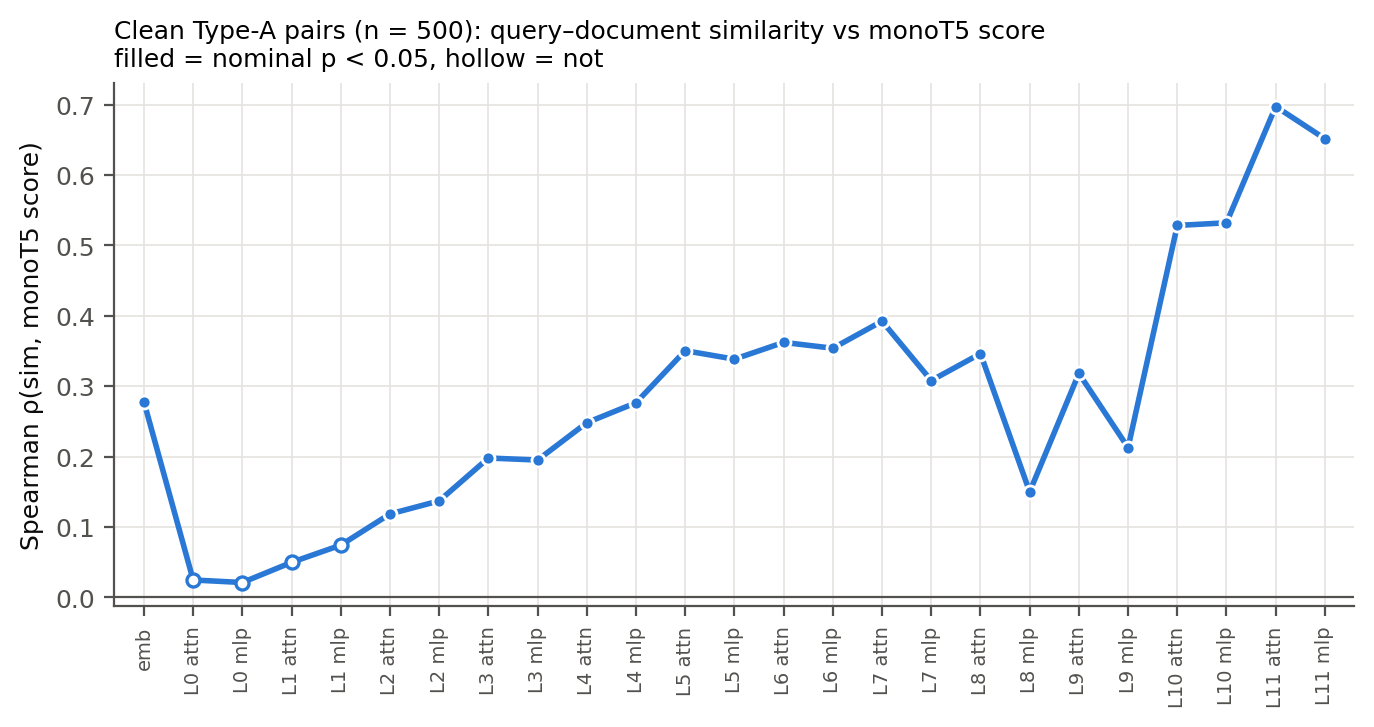
\includegraphics[width=0.85\textwidth]{outputs/plots/fig1_clean_rho.png}
\caption{Spearman $\rho(\qsim_{\mathrm{clean}}(c),\score_{\mathrm{clean}})$, 500 clean pairs.}
\end{figure}

\begin{itemize}[nosep]
  \item \textbf{Yes, and increasingly with depth.} At the embedding, $\rho=0.28$
        ($p=3\times10^{-10}$). This is a lexical-overlap signal: mean input embeddings
        are closer when query and passage share tokens.
  \item \textbf{Layers 0--1 wash it out} ($|\rho|\le0.07$, n.s.). After the first
        attention layer every position already mixes context, and the similarity
        level jumps from 0.45 to 0.80 for all pairs.
  \item \textbf{From layer 2 on, the association grows almost monotonically:}
        0.12 (L2), 0.25--0.28 (L4), 0.35--0.39 (L5--L7), then a jump to 0.53 at
        layer 10.
  \item \textbf{The maximum is $\rho=0.70$ at \texttt{L11\_post\_attn}.} The last MLP
        slightly weakens it (0.65).
  \item \textbf{Local dips follow MLP sublayers} (L7, L8, L9 post-MLP): the
        association is built by attention and partly undone by the MLPs.
\end{itemize}

\subsection{RQ2 --- Genuinely relevant documents are more query-similar at almost every depth}

\begin{figure}[H]
\centering
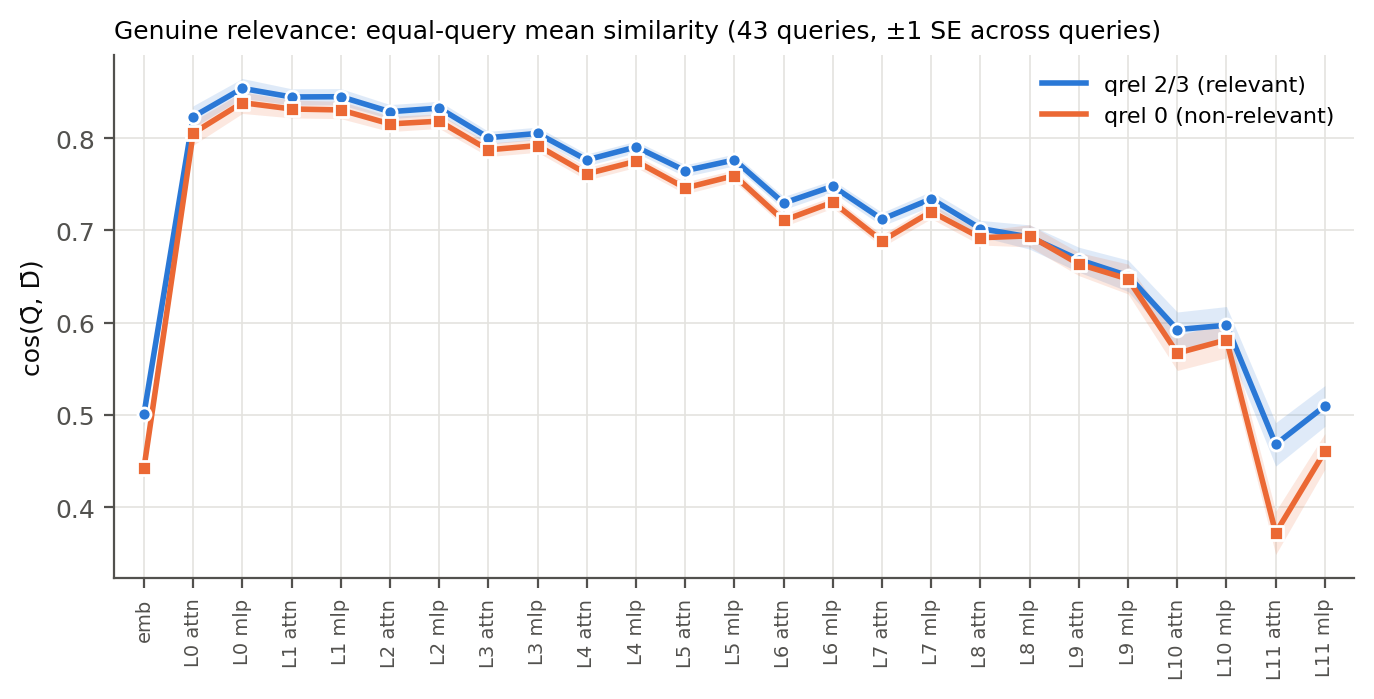
\includegraphics[width=0.85\textwidth]{outputs/plots/fig2_genuine_trajectory.png}\\
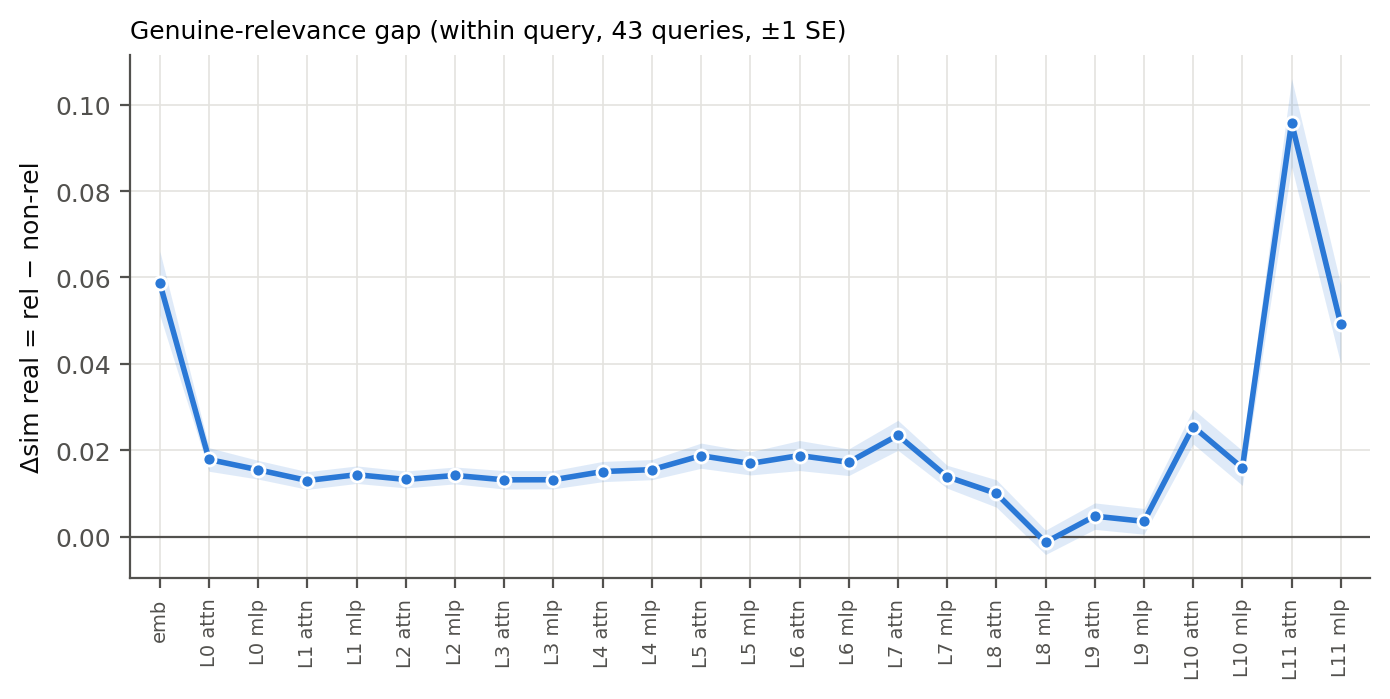
\includegraphics[width=0.85\textwidth]{outputs/plots/fig3_genuine_gap.png}
\caption{Top: equal-query mean similarity of qrel 2/3 vs qrel 0 documents. Bottom:
the within-query gap $\dsim_{\mathrm{real}}(c)$ ($\pm1$ SE across 43 queries).}
\end{figure}

\begin{itemize}[nosep]
  \item \textbf{The gap is positive at 24 of 25 checkpoints.} The exception is
        \texttt{L08\_post\_mlp} ($-0.001$, only 53\% of queries positive). At most
        checkpoints, 81--93\% of queries have a positive gap.
  \item \textbf{Separation already exists at the embedding} ($+0.059$), again the
        lexical signal.
  \item \textbf{Layer 0 attention compresses it} to $+0.018$ ($\dstep=-0.041$). It
        stays around $+0.013$--$0.024$ through layers 0--7.
  \item \textbf{Layers 8--9 nearly erase it}, mostly in the MLP sublayers.
  \item \textbf{Final-layer attention restores it most strongly:} $+0.026$ at
        \texttt{L10\_post\_attn} ($\dstep=+0.022$), then $+0.096$ at
        \texttt{L11\_post\_attn} ($\dstep=+0.080$, the single largest step).
  \item \textbf{The last MLP removes about half again} ($+0.049$).
\end{itemize}

The depth profile matches RQ1: the strongest genuine separation sits where the clean
similarity best predicts the score. For reference, the mean monoT5 score is
$-0.85$ for the relevant sample and $-9.66$ for the non-relevant one; these scores were
not used for selection.

\subsection{RQ3 --- The attack gap: negative at embeddings, small and positive mid-encoder, negative at layer 11}

\begin{figure}[H]
\centering
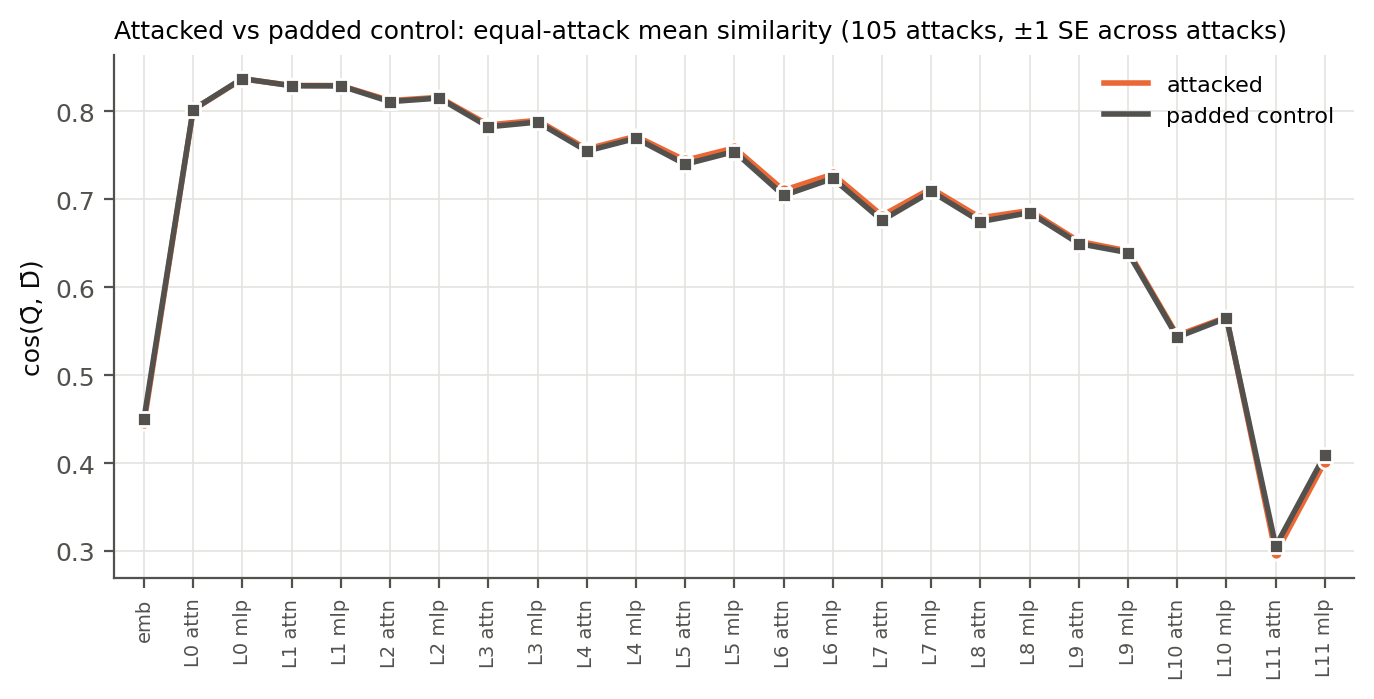
\includegraphics[width=0.85\textwidth]{outputs/plots/fig4_attack_control_trajectory.png}\\
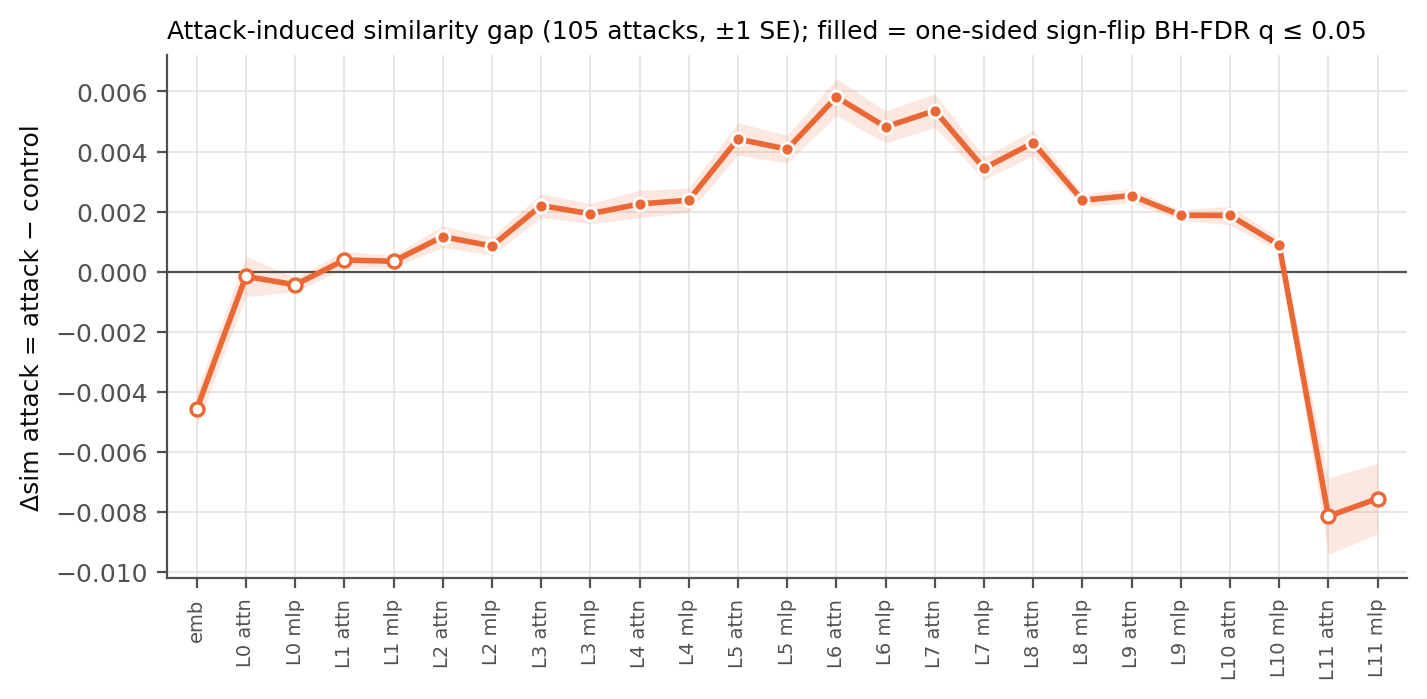
\includegraphics[width=0.85\textwidth]{outputs/plots/fig5_attack_gap.png}
\caption{Top: equal-attack mean similarity, attacked vs padded control. Bottom: the gap
$\dsim_{\mathrm{attack}}(c)$ ($\pm1$ SE across 105 attacks); filled markers pass
BH-FDR.}
\end{figure}

\begin{itemize}[leftmargin=*]
  \item \textbf{Is the gap present at the embedding?} Yes, but it is \emph{negative}:
        $-0.0046$, with only 26\% of attacks positive.
        \begin{itemize}[nosep]
          \item Injected tokens that are not query words pull the document mean away
                from the query.
          \item The effect scales with repetition count: $+0.0006$ for 1 repetition
                vs $-0.012$ for 5 (Figure~\ref{fig:brk}).
          \item At the embedding there is no ``artificial similarity''; there is
                dilution.
        \end{itemize}
  \item \textbf{Does it accumulate?}
        \begin{itemize}[nosep]
          \item Layer 0 attention cancels the dilution (${\approx}0$).
          \item The gap then turns positive and grows to a plateau of $+0.004$ to
                $+0.006$ at layers 5--7. The peak is $+0.0058$ at
                \texttt{L06\_post\_attn}, where 97\% of attacks are positive; at
                \texttt{L07\_post\_attn} 100\% are.
          \item It then decays through layers 8--10 and \emph{reverses} at layer 11
                ($-0.0081$ at \texttt{L11\_post\_attn}, $-0.0076$ at
                \texttt{L11\_post\_mlp}; only 15--18\% of attacks positive).
        \end{itemize}
  \item \textbf{BH-FDR (25 tests, one-sided):} the positive gap is significant at all
        18 checkpoints from \texttt{L02\_post\_attn} to \texttt{L10\_post\_mlp}
        ($q\le0.004$). It is not significant at the embedding, at layers 0--1, or at
        layer 11. The embedding and layer-11 gaps are negative, so the one-sided test
        cannot reject there, and no two-sided test was pre-registered.
  \item \textbf{Magnitude:} the significant mid-encoder gap is small in absolute terms.
        It is $\le0.006$ cosine, against a spread of 0.30--0.80 in the similarity
        levels themselves.
\end{itemize}

\begin{figure}[H]
\centering
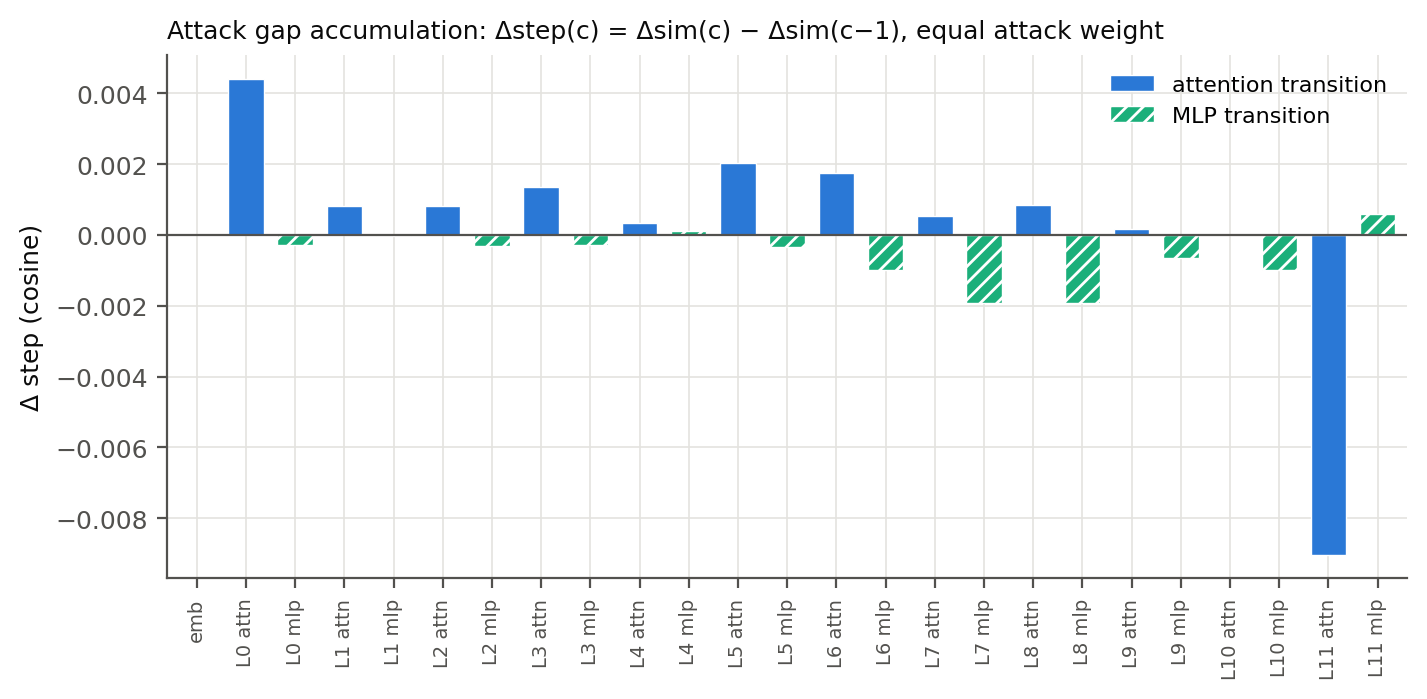
\includegraphics[width=0.85\textwidth]{outputs/plots/fig6_attack_accumulation.png}
\caption{Attack gap accumulation $\dstep_{\mathrm{attack}}(c)$, attention vs MLP transitions.}
\end{figure}

\textbf{Attention or MLP?} The gap is built by attention and eroded by the MLPs.
\begin{itemize}[nosep]
  \item Summed over the 12 layers, attention steps contribute $+0.0040$ (positive
        attention steps $+0.0131$) and MLP steps $-0.0070$ (positive MLP steps only
        $+0.0007$).
  \item Most layers show a positive attention step followed by a negative MLP step.
  \item The layer-11 reversal happens in the final \emph{attention} sublayer
        ($\dstep=-0.0090$), the same sublayer where the genuine gap grows most.
\end{itemize}

\subsection{RQ4 --- Attacks that raise similarity more also raise the score more}

\begin{figure}[H]
\centering
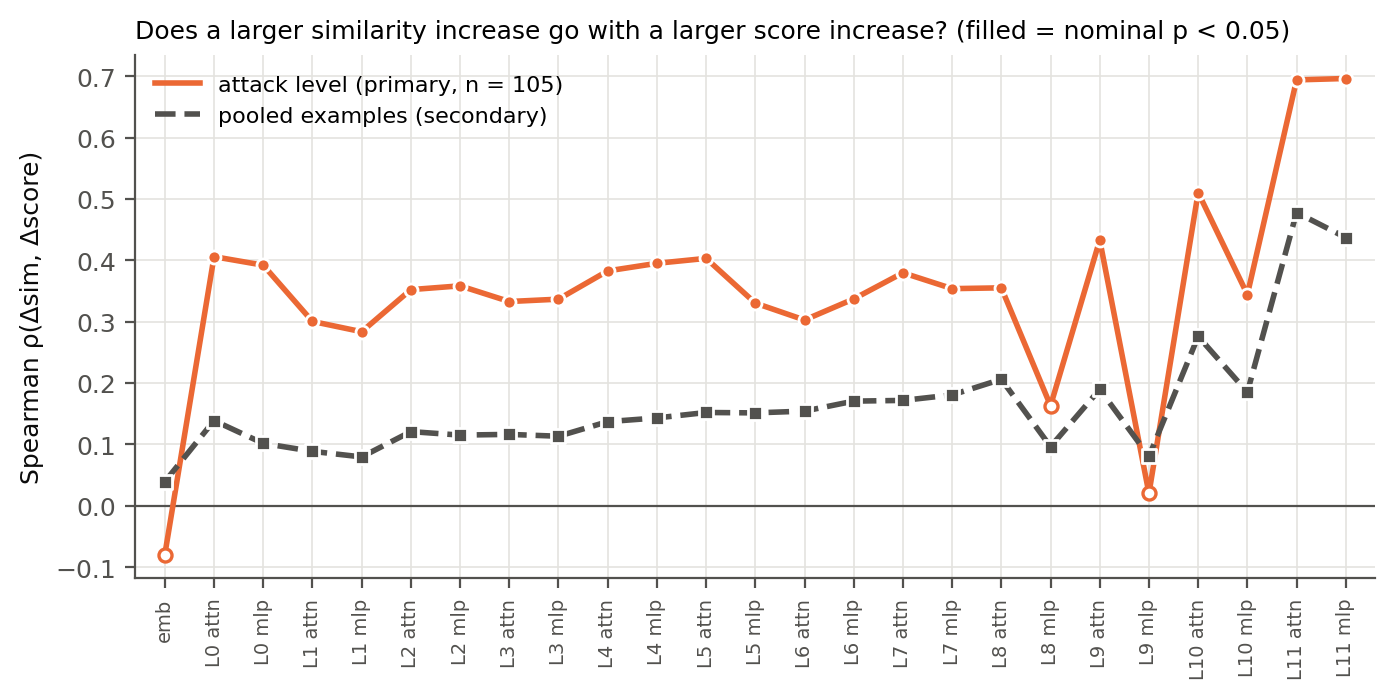
\includegraphics[width=0.85\textwidth]{outputs/plots/fig9_delta_sim_vs_delta_score.png}
\caption{Spearman across the 105 attacks between the attack-mean $\dsim$ and the
attack-mean $\Delta\score$ (primary; filled = nominal $p<0.05$), and the pooled
example-level Spearman (secondary, dashed).}
\end{figure}

\begin{itemize}[nosep]
  \item \textbf{The attack-level association is positive from layer 0 onward:}
        $\rho=0.30$--$0.43$ through layers 0--9 (nominal $p<0.01$ except
        \texttt{L08\_post\_mlp} and \texttt{L09\_post\_mlp}), $0.51$ at
        \texttt{L10\_post\_attn}, and $0.69$--$0.70$ at layer 11.
  \item \textbf{It is absent at the embedding} ($-0.08$).
  \item \textbf{The pooled example-level association is weaker}
        ($\rho\le0.48$, largest at layer 11).
\end{itemize}

The layer-11 association and the \emph{negative} mean layer-11 gap are not in
conflict. They reflect a split within the attack family:

\begin{itemize}[nosep]
  \item Only \textbf{12 of 105 attacks raise the mean score}. All of them are
        \emph{relevant} or \emph{information} injected at the start or end. The five
        strongest are \texttt{information\_start\_5} ($\overline{\Delta\score}=+0.38$),
        \texttt{relevant\_start\_5} ($+0.36$), \texttt{relevant\_start\_4},
        \texttt{information\_start\_4} and \texttt{information\_end\_5}.
  \item These attacks have a \emph{positive} layer-11 gap (mean $+0.008$;
        \texttt{information\_start\_5} $+0.019$) and the largest mid-encoder gaps
        (mean $+0.019$ at \texttt{L06\_post\_attn}, 3$\times$ the family average).
  \item \emph{Random}-position attacks lower the score the most (e.g.
        \texttt{true\_random\_5} $-0.30$, \texttt{relevant\_random\_5} $-0.29$). They
        also lower the layer-11 similarity the most ($-0.02$ to $-0.06$).
\end{itemize}

\subsection{Descriptive breakdowns}

\begin{figure}[H]
\centering
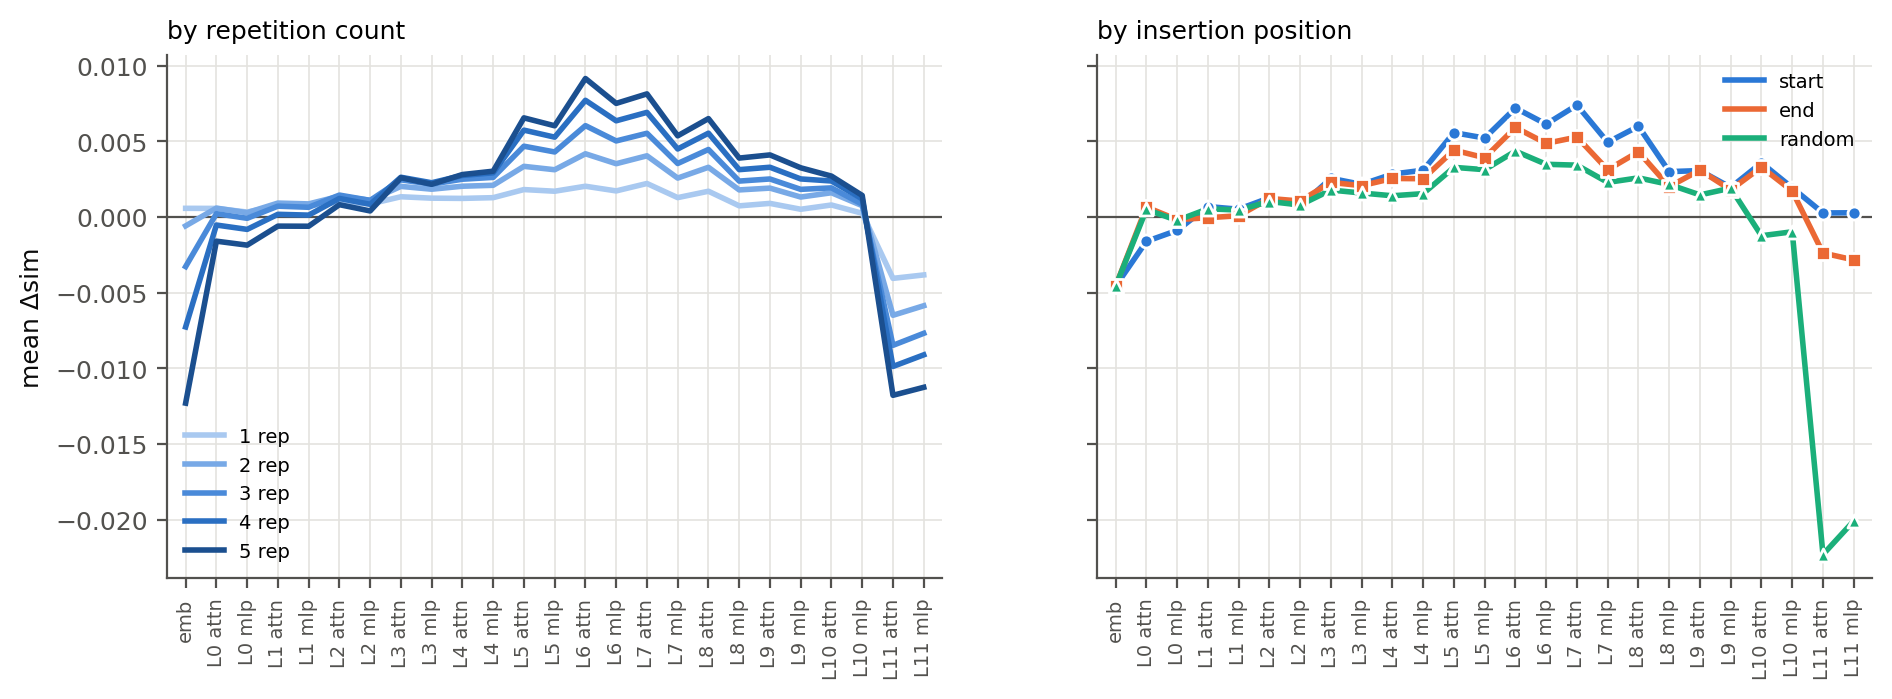
\includegraphics[width=\textwidth]{outputs/plots/figS2_breakdown_reps_position.png}\\
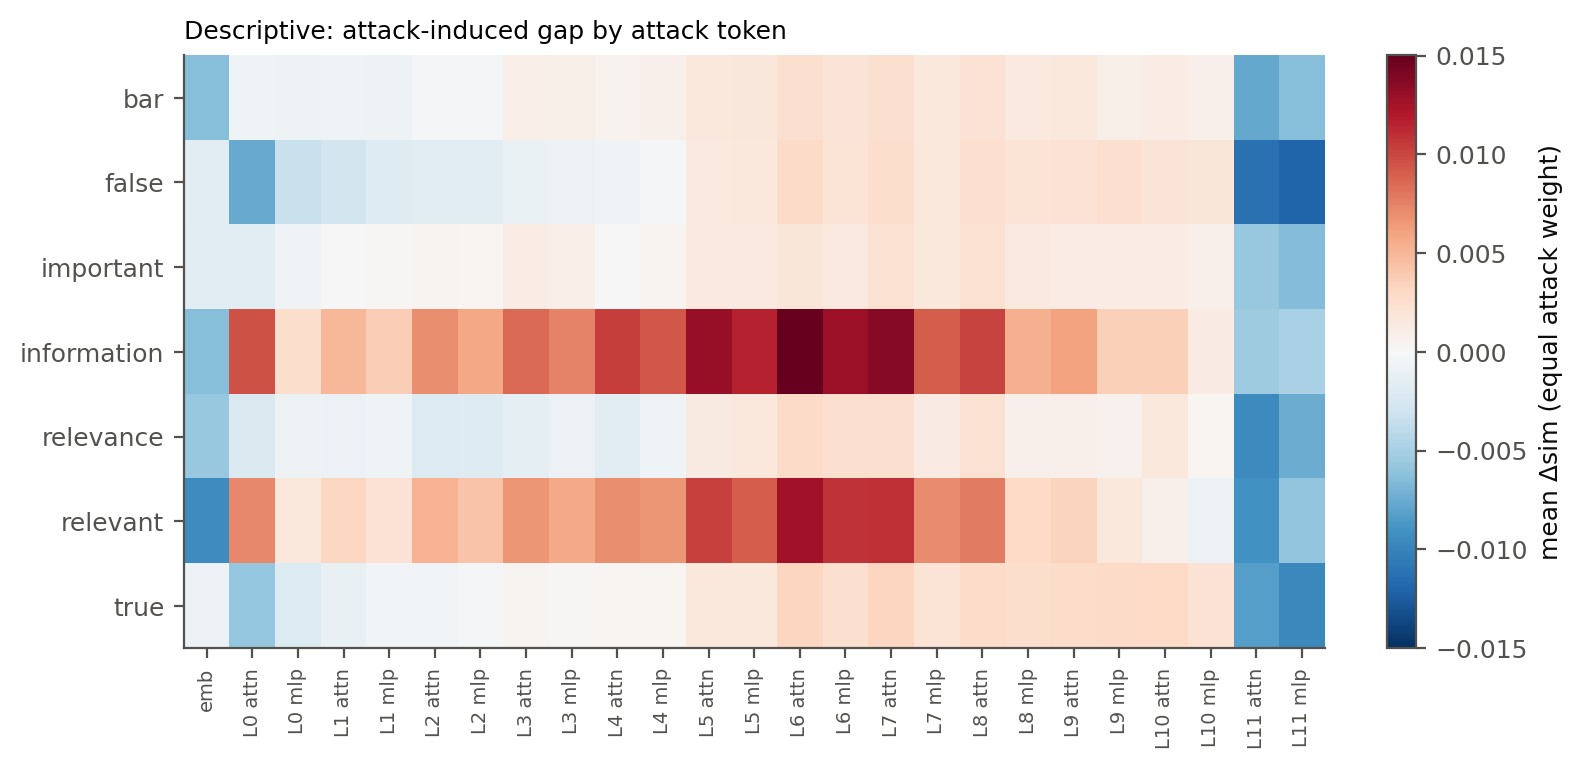
\includegraphics[width=0.85\textwidth]{outputs/plots/figS1_breakdown_token.png}
\caption{Equal-weight $\dsim$ by repetition count, insertion position and attack token
(descriptive; no additional tests).}
\label{fig:brk}
\end{figure}

\begin{itemize}[nosep]
  \item \textbf{Repetitions amplify every phase monotonically:} more embedding
        dilution, a larger mid-encoder gap, and a more negative layer-11 gap.
  \item \textbf{Position mainly matters at layer 11.} Start is about $+0.0003$, end
        $-0.003$, random $-0.02$.
  \item \textbf{Token:} \emph{information} and \emph{relevant} produce 4--6$\times$
        the mid-encoder gap of the other five tokens (L06: $+0.015$/$+0.013$ vs
        $+0.002$--$0.003$). They are also the only tokens with a near-zero or positive
        mean score change.
\end{itemize}

\subsection{Genuine vs adversarial: same sublayer mechanics, different depth profile}

\begin{figure}[H]
\centering
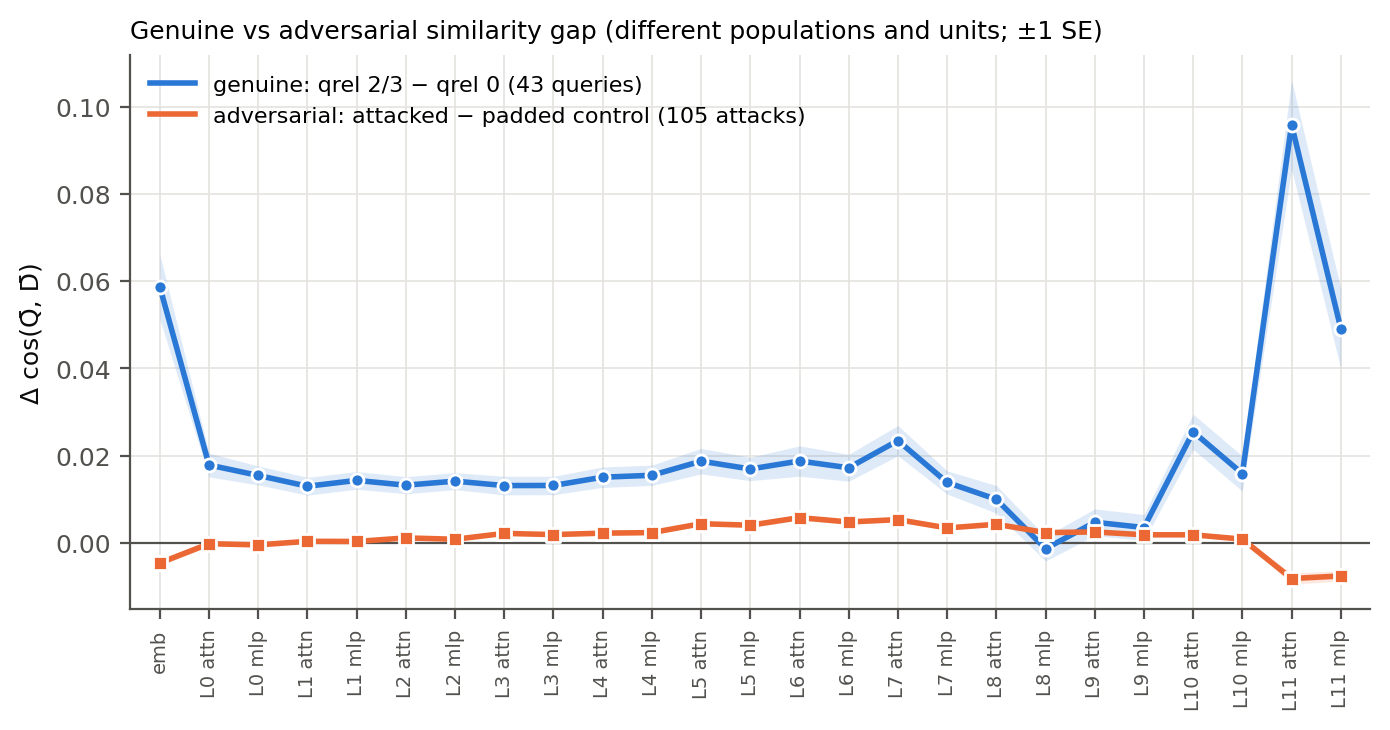
\includegraphics[width=0.85\textwidth]{outputs/plots/fig7_genuine_vs_attack_gap.png}\\
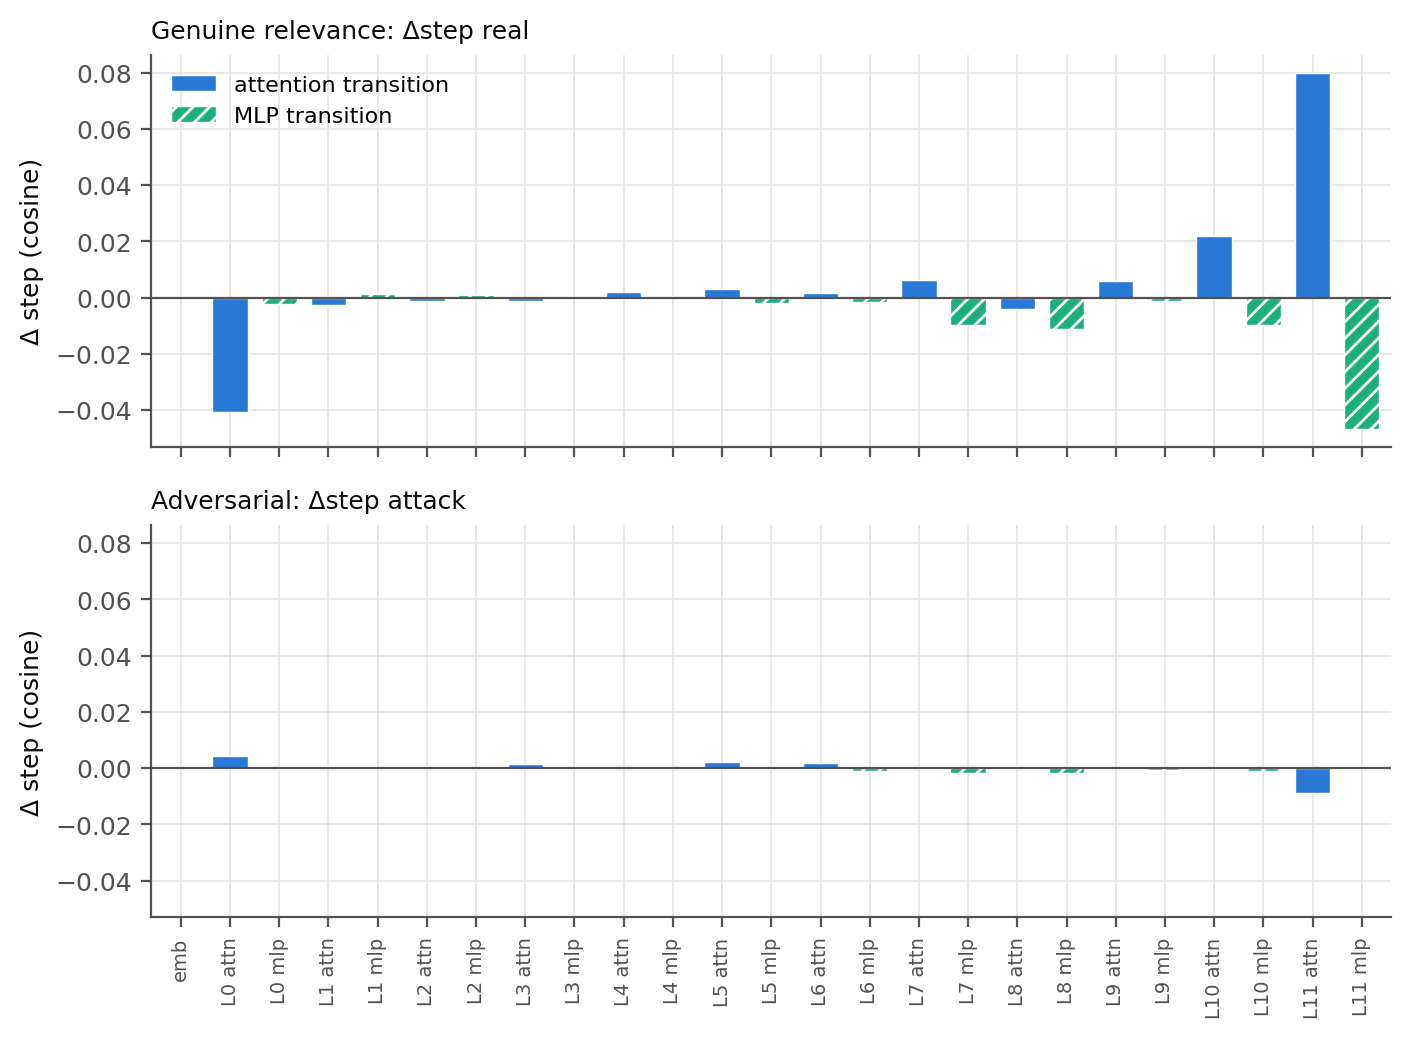
\includegraphics[width=0.85\textwidth]{outputs/plots/fig8_genuine_vs_attack_steps.png}
\caption{Top: $\dsim_{\mathrm{real}}$ and $\dsim_{\mathrm{attack}}$ on one axis.
Bottom: $\dstep_{\mathrm{real}}$ and $\dstep_{\mathrm{attack}}$ (shared $y$). The two
trajectories come from different populations and units (queries vs attacks).}
\end{figure}

\begin{enumerate}[leftmargin=*]
  \item \textbf{Both positive?} At 19 of 25 checkpoints (layers 1--10 except
        \texttt{L08\_post\_mlp}). They disagree at the embedding (real $+$, attack
        $-$), at \texttt{L00} (attack $\approx0$), and at both layer-11 checkpoints
        (real largest, attack negative).
  \item \textbf{Same depths?} Only partly. Both are positive through the middle
        encoder. The genuine gap's defining features, however, are its lexical
        embedding gap and its layer-11 surge, and at both points the average attack
        goes the other way. Across the 25 checkpoints the two trajectories are
        \emph{anti}-correlated (Pearson $-0.77$, descriptive), driven by those
        endpoints.
  \item \textbf{Same sublayers?} Qualitatively yes. For both, attention transitions
        build the gap and MLP transitions erode it.
        \begin{itemize}[nosep]
          \item Genuine: attention $+0.072$ (positive attention steps $+0.121$), MLP
                $-0.081$ (positive MLP steps $+0.003$).
          \item Attack: attention $+0.0040$, MLP $-0.0070$.
        \end{itemize}
        The step profiles are nonetheless anti-correlated (Pearson $-0.74$), because
        at \texttt{L11\_post\_attn} the genuine step is $+0.080$ and the attack step
        is $-0.009$.
  \item \textbf{Magnitude.} In layers 2--10 the family-average attack gap is roughly
        $\frac14$--$\frac13$ of the genuine gap. For the strongest successful attacks
        it is comparable to or larger than the genuine gap in the middle layers
        (\texttt{information\_start\_5} $+0.026$ vs genuine $+0.019$ at
        \texttt{L06\_post\_attn}). At layer 11 it stays far below: $+0.019$ vs
        $+0.049$ at \texttt{L11\_post\_mlp}. The family-average final ratio
        attack/real is $-0.15$ (secondary descriptive quantity).
\end{enumerate}

% =====================================================================
\section{Answers to the Research Questions}
% =====================================================================

\begin{enumerate}[leftmargin=*]
  \item \textbf{Clean similarity vs score:} yes. Spearman $\rho$ is up to 0.70 and
        significant (nominal $p<0.05$) at 21 of 25 checkpoints.
  \item \textbf{Where does it emerge?} A lexical component appears at the embedding
        (0.28). It vanishes in layers 0--1, rebuilds from layer 2, and is strongest in
        layers 10--11 (0.53--0.70).
  \item \textbf{Are qrel 2/3 documents more query-similar than qrel 0?} Yes, at 24 of
        25 checkpoints, in 81--93\% of queries at most depths.
  \item \textbf{Where does genuine separation emerge?} Already at the embedding
        ($+0.059$). It is maintained at about $+0.015$ through the middle layers,
        nearly vanishes at layers 8--9, and peaks at \texttt{L11\_post\_attn}
        ($+0.096$).
  \item \textbf{Are attacked documents more query-similar than padded controls?} Only
        in layers 2--10: a small but highly consistent gap of $\le0.006$, passing
        BH-FDR at 18 checkpoints. They are \emph{less} similar at the embedding and at
        layer 11.
  \item \textbf{Is the attack gap present at the embedding?} No positive gap. The
        embedding shows dilution ($-0.005$, growing with repetitions).
  \item \textbf{Does attack similarity accumulate?} Yes, from layer 1 to layers 6--7.
        It then decays and reverses at layer 11.
  \item \textbf{Attention or MLP?} Attention transitions build the attack gap and MLP
        transitions erode it. The layer-11 reversal is an attention step.
  \item \textbf{Genuine accumulation pattern?} Same sublayer division of labour.
        Different depths: the genuine gap is carried from the embedding and surges in
        layer-11 attention.
  \item \textbf{Does the attack trajectory resemble the genuine one?} Only in the
        middle encoder, and only weakly on average. Overall the trajectories are
        anti-correlated. The minority of score-raising attacks resemble genuine
        relevance more: positive at layer 11, but much smaller.
  \item \textbf{Do larger similarity changes go with larger score changes?} Yes,
        across attacks: $\rho\approx0.3$--$0.4$ mid-encoder and $0.70$ at layer 11.
  \item \textbf{Which attack checkpoints survive BH-FDR?} All 18 from
        \texttt{L02\_post\_attn} through \texttt{L10\_post\_mlp}. None of
        \texttt{embedding}, \texttt{L00}, \texttt{L01} or \texttt{L11} survive.
\end{enumerate}

% =====================================================================
\section{Supplementary Analyses: Similarity Levels, Important Heads and the Decoder}
% =====================================================================

The primary analyses compare gaps (relevant $-$ non-relevant, attack $-$ control) over
the full, unfiltered attack family. This section asks a complementary, descriptive
question: in absolute terms, does a \emph{successful} attacked input look like a genuinely
relevant document? Four populations are compared (stages 06--12):

\begin{itemize}[nosep]
  \item clean, genuinely relevant (qrel 2/3) and clean, non-relevant (qrel 0): the
        balanced qrel sample of 43 queries, averaged within query, then equal weight
        per query, $\pm1$ SE across queries;
  \item attacked, \textbf{successful}: the 18,906 examples with example-level
        $\Delta\score=\score_{\mathrm{attack}}-\score_{\mathrm{control}}>0$;
  \item attacked, \textbf{unsuccessful}: the 33,572 examples with $\Delta\score\le0$.
\end{itemize}

For both attack groups, only the attacked input itself is used, with the injected tokens
in the document span. Examples are averaged within each attack, then the attacks are
weighted equally, with $\pm1$ SE across attacks. All 105 attacks contain both successful
(80--405 per attack) and unsuccessful (95--420) examples.

The success split is used \emph{only} in these descriptive plots. Throughout,
\textbf{colour marks the population}: blue for the clean judged documents, orange for the
attacked inputs. \textbf{Line style marks the outcome}: solid for relevant or successful,
dashed for non-relevant or unsuccessful.

\subsection{Encoder: similarity levels at the 25 checkpoints}

\begin{figure}[H]
\centering
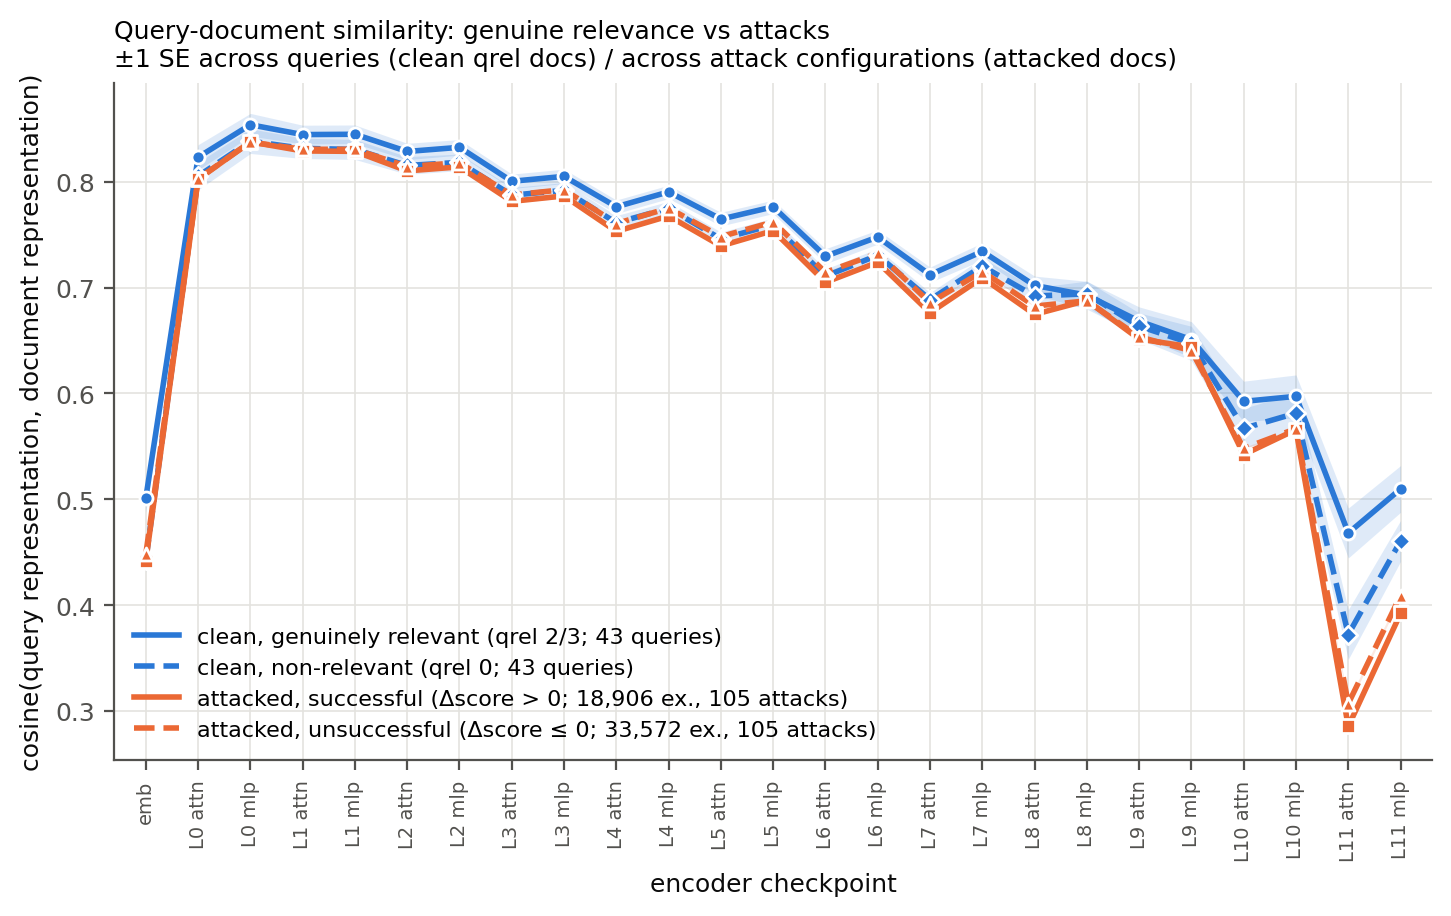
\includegraphics[width=0.9\textwidth]{outputs/plots/fig_successful_attacks_vs_genuine_similarity.png}
\caption{Absolute $\cos(Q_c,D_c)$ at the 25 encoder checkpoints for the four
populations (the same metric as Section~2).}
\label{fig:enc_levels}
\end{figure}

\begin{itemize}[nosep]
  \item \textbf{Layers 0--9:} the four curves move together within about 0.03.
        Genuinely relevant documents are always on top. The other three are nearly
        indistinguishable.
  \item \textbf{Layers 10--11:} the populations separate. At \texttt{L11\_post\_attn}
        the values are 0.47 (relevant), 0.37 (non-relevant), 0.31 (unsuccessful) and
        0.29 (successful). At \texttt{L11\_post\_mlp} they are 0.51, 0.46, 0.41 and
        0.39.
  \item \textbf{Successful attacks do not reach even the non-relevant level} at the
        final layer. They are marginally \emph{below} the unsuccessful ones.
\end{itemize}

This does not contradict RQ4. RQ4 concerns each document's \emph{increase} over its own
padded control; Figure~\ref{fig:enc_levels} concerns absolute levels. One plausible
reason the levels are low is selection: attacks mostly succeed on documents that started
out less relevant.

\subsection{Important encoder heads}

For each of the 18 canonical important encoder heads (Exp~13
\texttt{encoder\_senders.json}), the same metric is applied to that head's own 64-d
output before \texttt{o\_proj}. It is pooled over query-text positions and over document
positions, and the two pooled vectors are compared by cosine.

\begin{figure}[H]
\centering
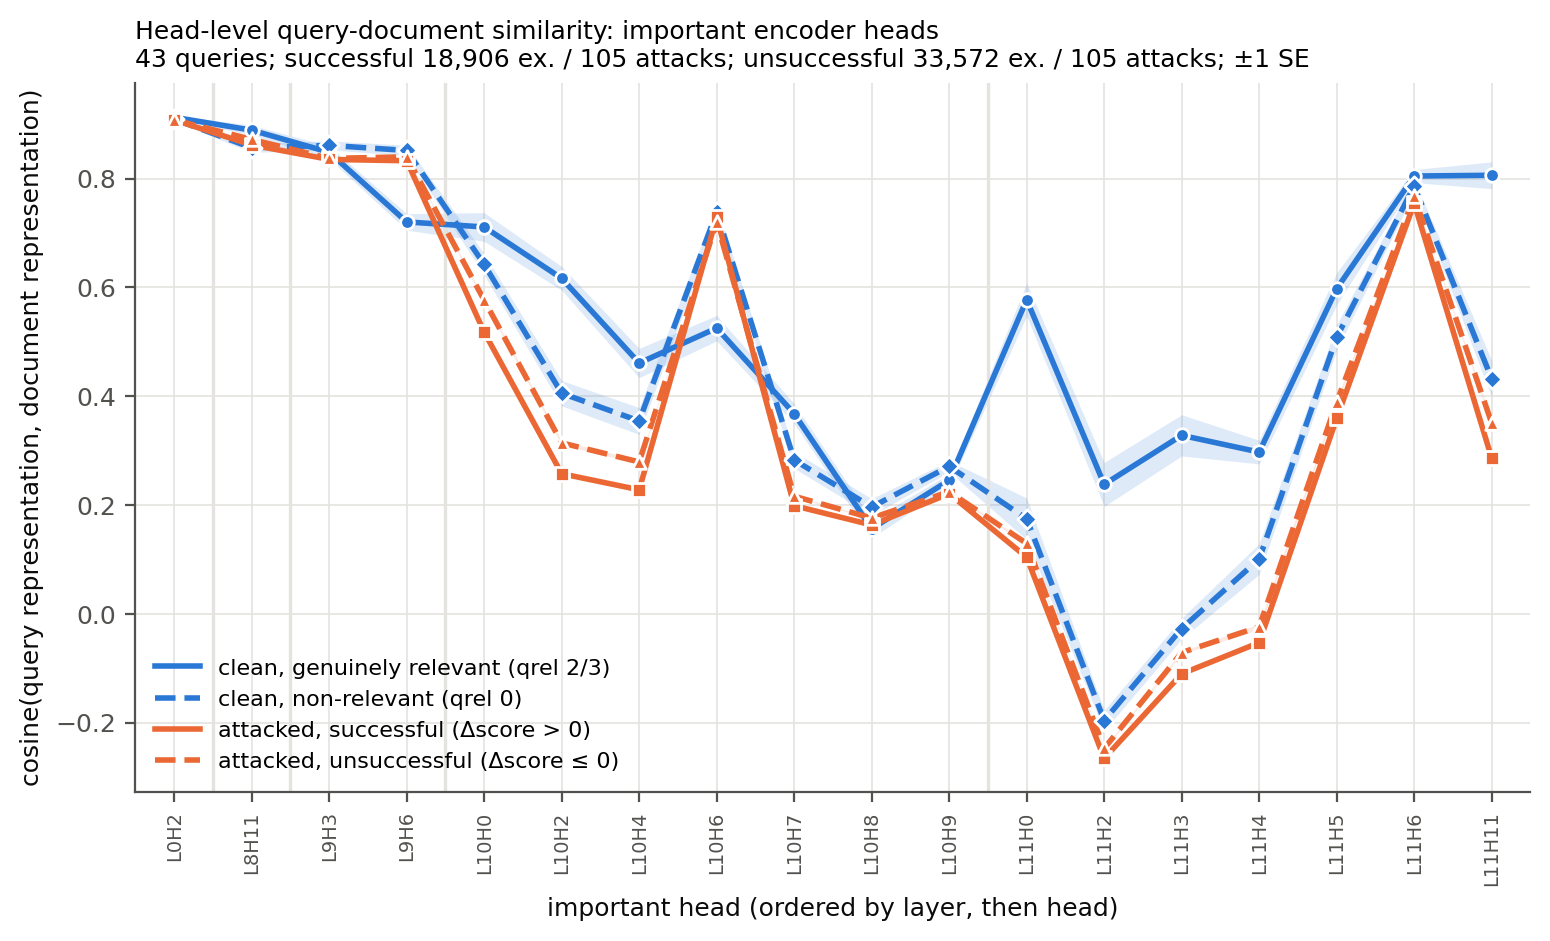
\includegraphics[width=0.9\textwidth]{outputs/plots/fig_heads_encoder_four_populations.png}
\caption{Head-level query--document similarity at the 18 important encoder heads
(ordered by layer, then head).}
\label{fig:enc_heads}
\end{figure}

\begin{itemize}[nosep]
  \item \textbf{Heads that separate genuine relevance most:} \texttt{L11H2} ($+0.43$
        relevant $-$ non-relevant), \texttt{L11H0} ($+0.40$), \texttt{L11H11}
        ($+0.37$), \texttt{L11H3} ($+0.36$) and \texttt{L10H2} ($+0.21$).
  \item \textbf{Attacks at those heads:} both attack groups sit with or below the
        non-relevant documents. At \texttt{L11H11}, for example, the values are 0.81
        (relevant), 0.43 (non-relevant), 0.35 (unsuccessful) and 0.29 (successful).
  \item \textbf{Two heads run the other way:} at \texttt{L9H6} and \texttt{L10H6},
        relevant documents are \emph{less} query-similar than non-relevant ones
        ($-0.13$, $-0.21$). Attacks follow the non-relevant level there too.
  \item \textbf{Successful vs unsuccessful:} successful attacks are closer to genuine
        relevance than unsuccessful ones at only 3 of 18 heads. At the discriminating
        heads \texttt{L10H0}, \texttt{L10H2}, \texttt{L10H4} and \texttt{L11H11} they
        are 0.05--0.06 \emph{less} query-similar than unsuccessful attacks.
\end{itemize}

\subsection{Decoder}

At the first decoder step there is a single position. Query and document information
reaches it only through cross-attention, so the encoder metric cannot be applied
directly. Two decoder-side definitions are used.

\paragraph{Cross-attention messages (stages 07/08, per layer).} In each decoder layer the
cross-attention output (after \texttt{.o}, before the residual add) is split by source
span:
\[
m_S=\texttt{o}\Big(\textstyle\sum_{j\in S}P_{h,j}V_{h,j}\Big)_h .
\]
The plotted quantity is $\cos(m_{\mathrm{query}},m_{\mathrm{doc}})$. On every batch the
query, document and template parts together reproduce the cross-attention output to a
relative error $\le10^{-6}$.

\begin{figure}[H]
\centering
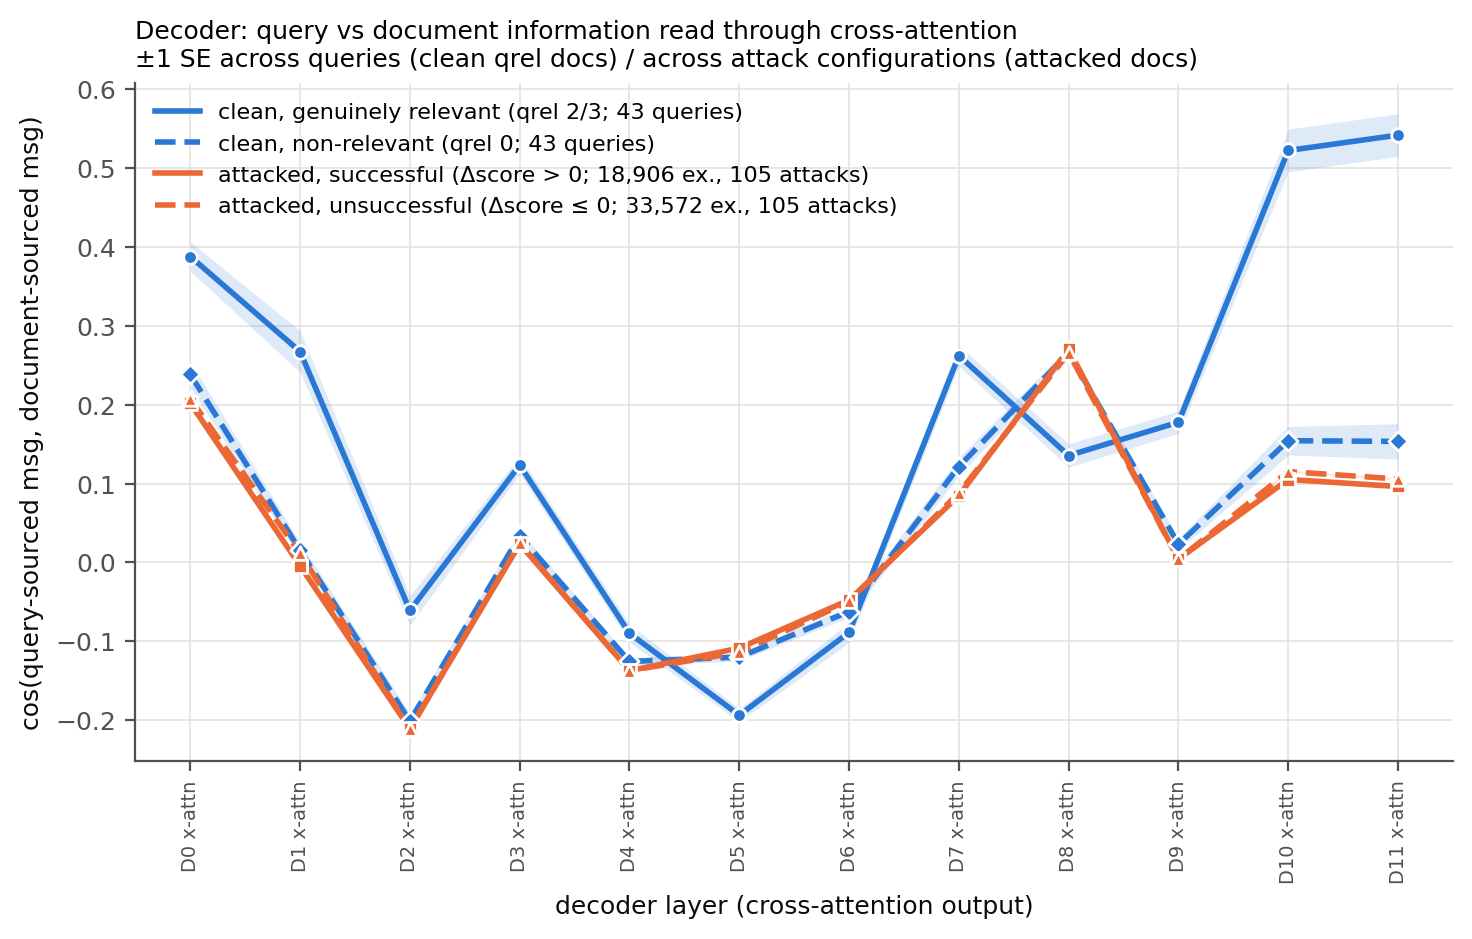
\includegraphics[width=0.85\textwidth]{outputs/plots/fig_decoder_message_similarity_four_populations.png}
\caption{Per decoder layer: cosine between the cross-attention message read from the
query text and the message read from the document.}
\label{fig:dec_msg}
\end{figure}

\begin{itemize}[nosep]
  \item \textbf{Genuine relevance separates most sharply in the last two decoder
        layers:} 0.52 (D10) and 0.54 (D11) for relevant documents, against 0.15 for
        non-relevant ones.
  \item \textbf{Both attack groups sit below the non-relevant documents there}
        (0.10--0.12).
  \item \textbf{Relevant documents are also clearly higher at D0, D1, D3, D7 and D9.}
        D8 is the one reversal: the non-relevant and both attack groups (0.27) are well
        above the relevant documents (0.14).
\end{itemize}

\paragraph{Residual-stream probe (stages 11/12, every sublayer).} The encoder is run once.
The first decoder step is then run twice from that output: once with cross-attention
restricted to the query-text positions (the decoder's representation of the query) and
once restricted to the document positions (its representation of the document). The
plotted quantity is $\cos(h_{\text{query-only}},h_{\text{doc-only}})$ of the decoder
residual state at 37 checkpoints: the embedding, then post self-attention, post
cross-attention and post MLP for each layer, with layer 11 taken before
\texttt{final\_layer\_norm}.

Restricting cross-attention renormalises the attention over the kept span, so each run
is a probe rather than the model's normal pass. As required, the two checkpoints before
any cross-attention are identical in both runs (maximum $|1-\cos|\approx10^{-16}$).

\begin{figure}[H]
\centering
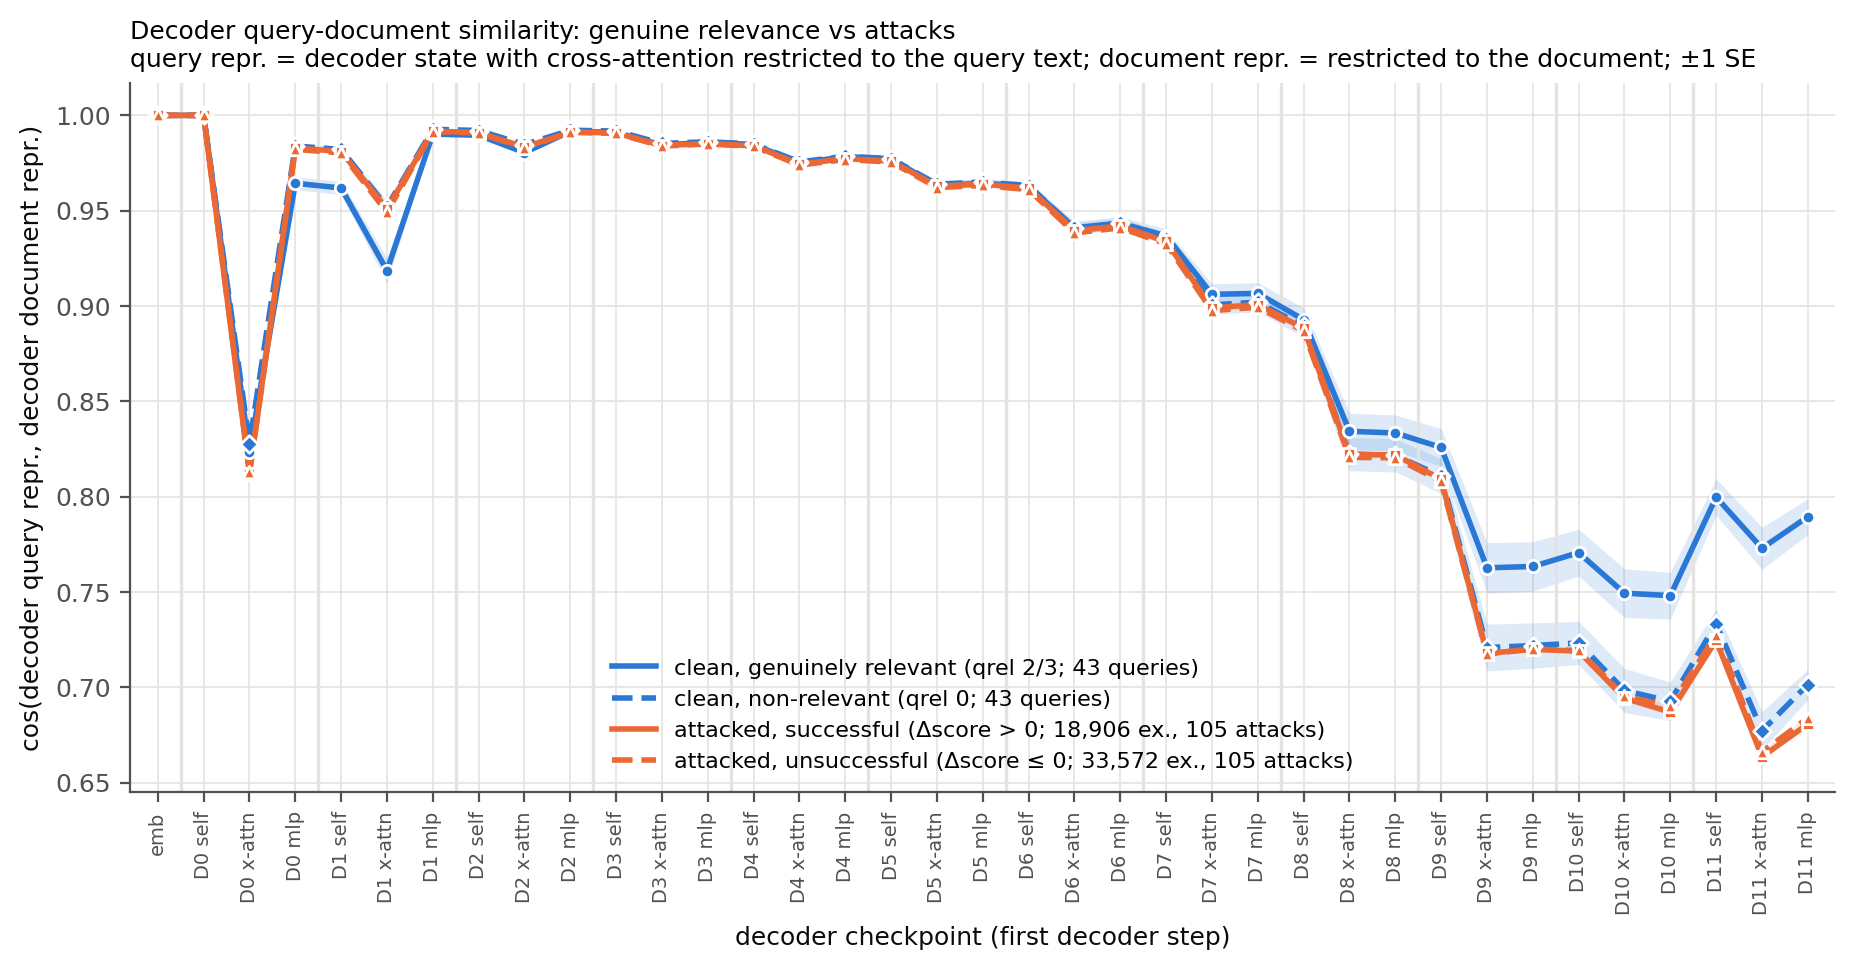
\includegraphics[width=\textwidth]{outputs/plots/fig_decoder_probe_similarity_four_populations.png}
\caption{Decoder residual-stream query--document similarity at every decoder sublayer.}
\label{fig:dec_probe}
\end{figure}

\begin{itemize}[nosep]
  \item \textbf{Layers 2--7:} all four groups stay at 0.93--0.99. The shared
        start-token embedding dominates the decoder residual stream there.
  \item \textbf{Early separation:} at layers 0--1, relevant documents already sit lower
        at the MLP and cross-attention steps (0.92 vs 0.95 after D1 cross-attention).
  \item \textbf{Late separation, mostly at cross-attention steps:} from D8 on, genuine
        relevance separates, growing at the D8, D9 and D11 cross-attention steps.
        After D11 cross-attention the values are 0.77 (relevant), 0.68
        (non-relevant), 0.67 (unsuccessful) and 0.66 (successful).
  \item \textbf{Attacks track the non-relevant documents} throughout, and end slightly
        below them.
\end{itemize}

\paragraph{Important decoder heads.} For the 31 canonical important decoder heads (Exp~13
\texttt{decoder\_receivers.json}; all cross-attention), the per-head query-sourced and
document-sourced 64-d contributions $\sum_{j\in S}P_{h,j}V_{h,j}$ at the first decoder
step are compared by cosine (Figure~\ref{fig:dec_heads}).

\begin{figure}[H]
\centering
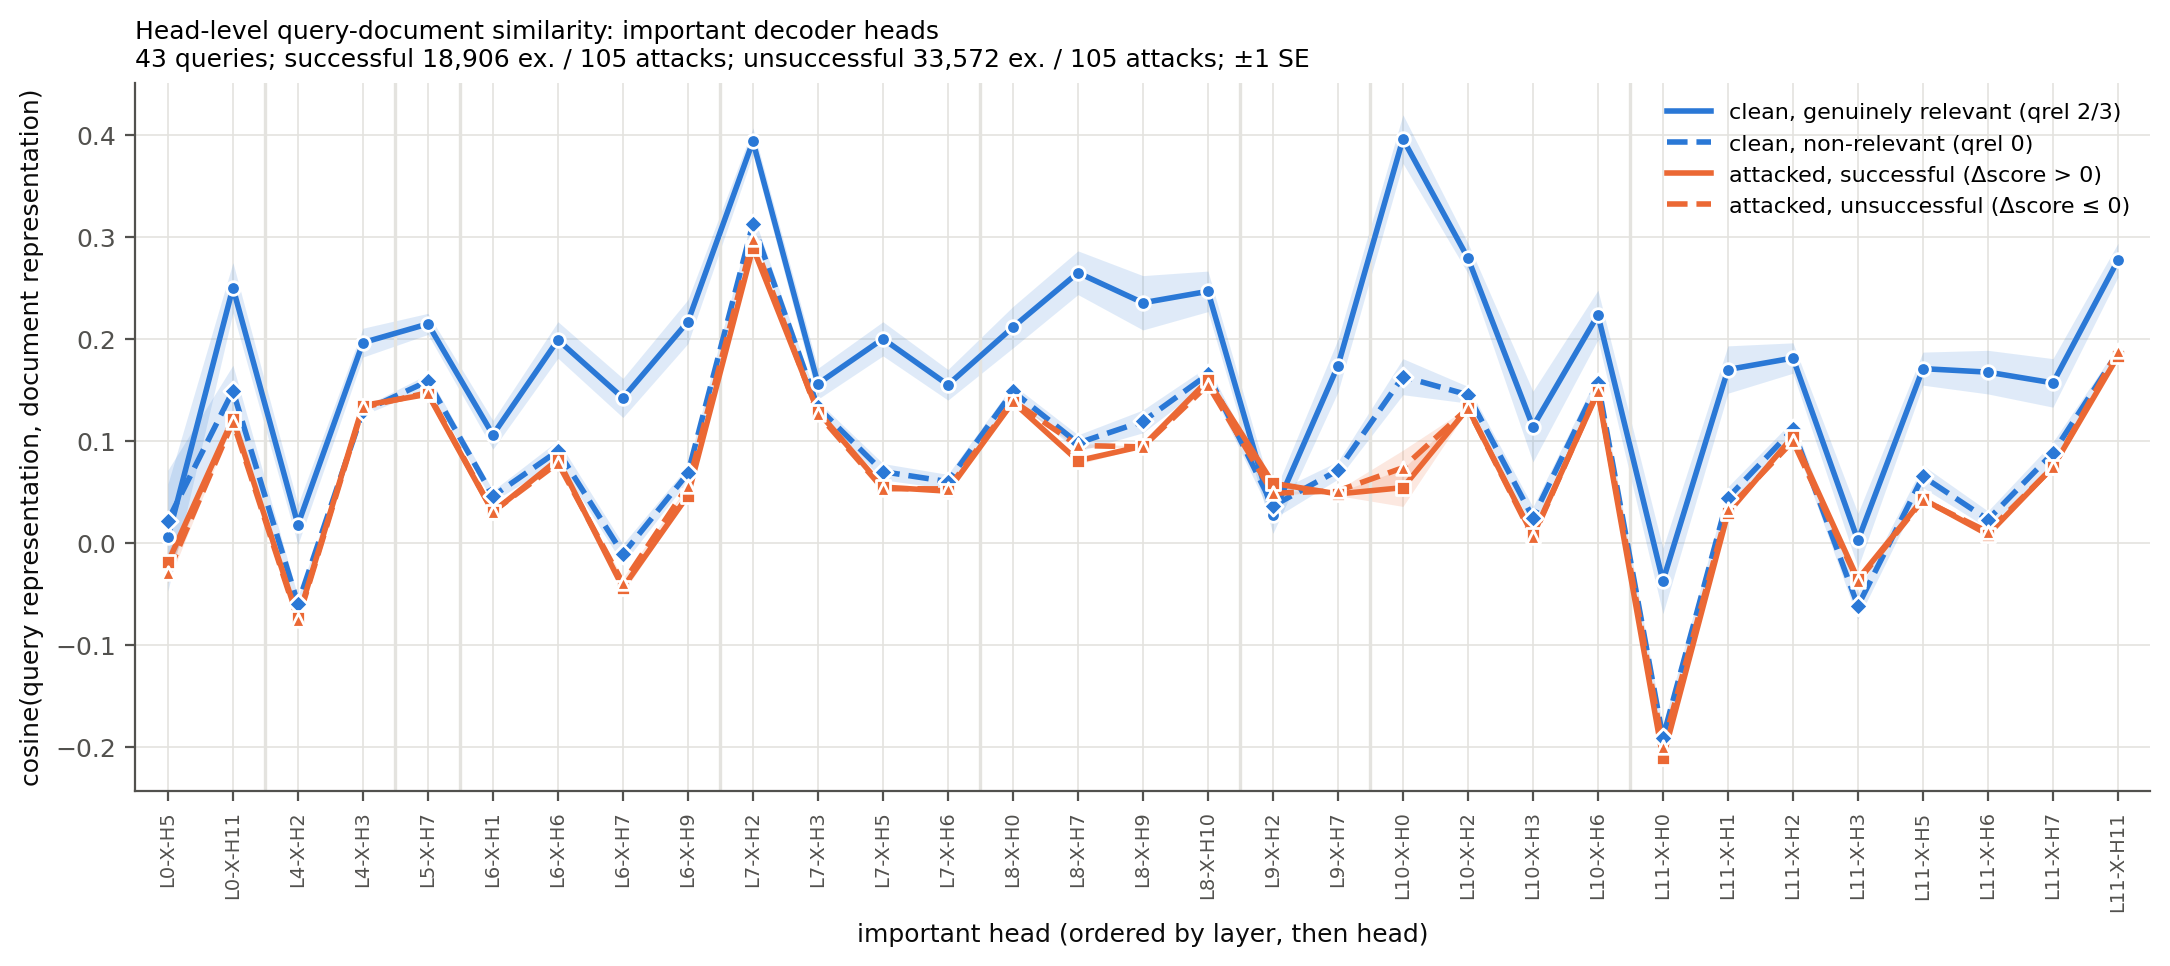
\includegraphics[width=\textwidth]{outputs/plots/fig_heads_decoder_four_populations.png}\\[4pt]
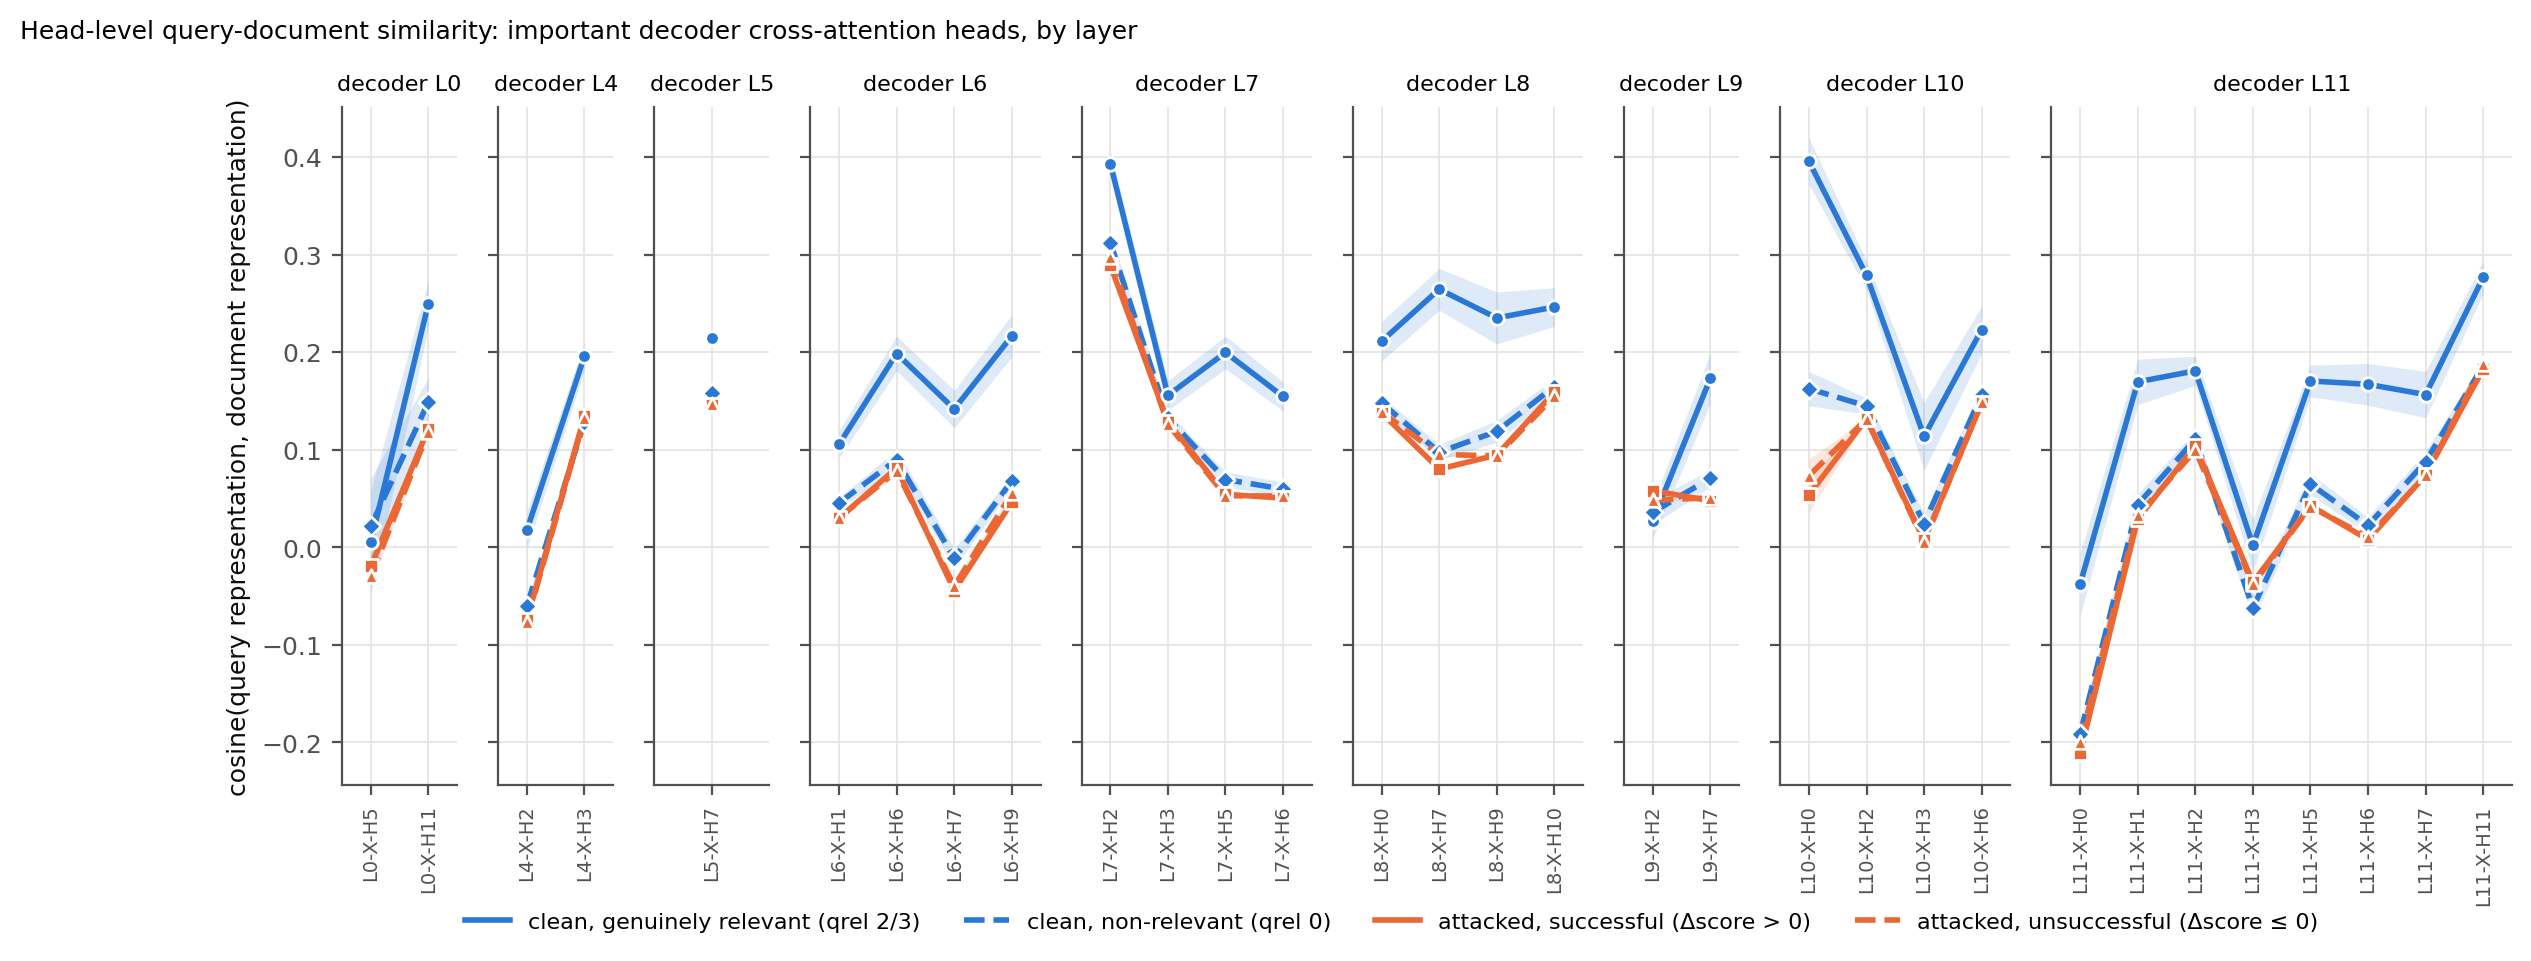
\includegraphics[width=\textwidth]{outputs/plots/fig_heads_decoder_four_populations_by_layer.png}
\caption{Head-level query--document similarity at the 31 important decoder
cross-attention heads (top: all heads; bottom: the same data split per decoder layer).}
\label{fig:dec_heads}
\end{figure}

\begin{itemize}[nosep]
  \item \textbf{Heads that separate relevant from non-relevant most:}
        \texttt{L10-X-H0} ($+0.23$), \texttt{L8-X-H7} ($+0.17$), \texttt{L11-X-H0}
        ($+0.15$), \texttt{L6-X-H7}, \texttt{L6-X-H9} and \texttt{L11-X-H6} ($+0.15$
        each).
  \item \textbf{Attacks sit at the non-relevant level at every head.} Successful and
        unsuccessful attacks never differ by more than 0.02.
\end{itemize}

The simplified two-line versions (genuine relevant vs successful attack only) are in
\texttt{outputs/plots/fig\_heads\_\{encoder,decoder\}\_genuine\_vs\_successful.png}.
All plotted numbers are in \texttt{outputs/04\_analysis/} and
\texttt{outputs/10\_head\_analysis/}.

\subsection{What the supplementary analyses add}

\begin{itemize}[nosep]
  \item \textbf{Successful attacks do not look like genuinely relevant documents} at any
        level examined: the encoder checkpoints, the important encoder heads, the
        decoder cross-attention messages, the decoder residual stream and the
        important decoder heads.
  \item \textbf{They look like clean non-relevant documents}, and in the late encoder
        and decoder slightly less query-similar still.
  \item \textbf{Successful and unsuccessful attacks are almost indistinguishable in
        these levels.} Where they differ, at late encoder heads, successful attacks are
        the \emph{less} similar group.
  \item \textbf{Implication:} whatever makes an attack succeed, it is not visible as
        genuine-relevance-like query--document similarity in absolute terms. That
        points away from ``the attack makes the document look relevant'' and towards a
        different route to the \texttt{true} logit. The earlier causal experiments
        located that route in late encoder heads and cross-attention.
  \item \textbf{Caveats:} these are level comparisons between different document
        sources (BM25-retrieved pairs vs the judged DL19 pool). The decoder
        residual-stream probe restricts cross-attention and is therefore not the
        model's normal pass. All results are descriptive.
\end{itemize}

% =====================================================================
\section{Interpretation and Discussion}
% =====================================================================

\paragraph{Positive findings.}
\begin{itemize}[nosep]
  \item Query--document similarity is a real internal correlate of monoT5's relevance
        judgement. It tracks the score on clean data, separates human-judged relevant
        from non-relevant documents, and is both largest and most predictive in the
        last encoder layer's attention.
  \item Keyword stuffing does leave a similarity signature: a small, very consistent
        mid-encoder increase that grows with repetition count and is largest for the
        tokens (\emph{relevant}, \emph{information}) and positions (start, end) that
        actually work.
  \item Across the attack family, the similarity change tracks the score change,
        most strongly at layer 11.
\end{itemize}

\paragraph{Null and negative findings.}
\begin{itemize}[nosep]
  \item Averaged over all 105 attacks, stuffing does \emph{not} make the final encoder
        representations more query-similar. The mean layer-11 gap is negative.
  \item At the embedding the injected tokens simply dilute the document mean.
  \item The average attack trajectory is anti-correlated with the genuine one.
  \item Consistent with this, the average attack in this unfiltered population
        \emph{lowers} the score: equal-attack mean $\Delta\score=-0.079$, and only 36\%
        of examples go up.
\end{itemize}

\paragraph{Real vs adversarial.}
\begin{itemize}[nosep]
  \item Genuine relevance starts from lexical overlap that is already visible in the
        input embeddings, and is amplified most by final-layer attention.
  \item Adversarial injection starts from dilution, gains a small mid-encoder
        similarity through attention, and loses it again in final-layer attention
        unless the attack is one of the few effective ones.
\end{itemize}
The strongest justified statement is therefore: \emph{artificial query--document
similarity is a representational signature of the effective attacks. It resembles the
genuine-relevance pattern in the middle encoder and weakly at layer 11, but is much
smaller than it, and it is not a general property of keyword stuffing.}

\paragraph{Relation to earlier experiments.} The depth profile of RQ4 fits the earlier
localisation. In Exps~1 and 11 the attack effect concentrates in late encoder
self-attention. Here, the layer-10/11 attention checkpoints are where similarity best
predicts the score, both on clean data and across attacks. Whether the similarity
change \emph{mediates} the score change cannot be decided here.

% =====================================================================
\section{Limitations and Threats to Validity}
% =====================================================================

\begin{itemize}[leftmargin=*]
  \item \textbf{No causal claim.} Similarity is measured, not manipulated. A
        correlation between $\dsim$ and $\Delta\score$ (RQ4) could arise from a
        common cause, for example how strongly the injected token interacts with the
        query in attention. Testing mediation would require an intervention that
        removes the similarity gap (e.g. patching the important heads) and checks
        whether the score change follows.
  \item \textbf{Different populations.} The genuine gap compares \emph{different
        documents} for the same query. The attack gap compares the \emph{same passage}
        with and without injected tokens. Magnitudes are not directly comparable, and
        the genuine gap includes lexical-overlap differences that the attack gap by
        construction does not.
  \item \textbf{Pooling choices.} Mean-pooling and including the attack tokens in $D$
        are locked design choices (DECISIONS~2--7). The embedding-level dilution is
        partly a direct consequence of including non-query tokens in the mean. A
        passage-only pool would answer a different question.
  \item \textbf{Unfiltered attacks.} The population deliberately includes the
        majority of attacks that lower the score. Family-level averages are therefore
        dominated by ineffective attacks. The per-attack table and RQ4 separate them.
  \item \textbf{One-sided test.} The sign-flip tests only positive gaps. The negative
        embedding and layer-11 gaps are reported descriptively (SE bands, fraction of
        attacks), not tested.
  \item \textbf{Supplementary decoder probe.} The decoder residual-stream comparison
        restricts cross-attention to one span per run (renormalised attention), so it
        describes hypothetical decoder passes. The cross-attention message split, by
        contrast, is an exact decomposition of the normal pass.
  \item \textbf{Qrel sample.} The genuine-relevance analysis is descriptive. The
        per-query gaps are saved (\texttt{qrel\_per\_query\_trajectory.csv}) for later
        inference. The qrel documents are the judged DL19 pool, not the BM25 pairs used
        for the attacks.
\end{itemize}

% =====================================================================
\section{Reproducibility}
% =====================================================================

\begin{lstlisting}
cd patch_code/analysis/16_monot5_artificial_query_document_similarity
bash bash/run_tests.sh                       # 45 pytest tests (CPU)
bash bash/run_smoke_test.sh                  # smoke pipeline -> outputs_smoke/
# full run (SLURM job 1420511, L40, ~6 min end-to-end):
cd /home/ghoummaid/IR && bash run_job.sh --job-name monot5_exp16_similarity \
  --gpu-type L40 --gpu-count 1 --cores 8 --time 24:00:00 \
  --output-dir ./patch_code/analysis/16_monot5_artificial_query_document_similarity/slurm_logs \
  --command "cd /home/ghoummaid/IR/patch_code/analysis/16_monot5_artificial_query_document_similarity && bash bash/run_all.sh configs/default.yaml"
# supplementary stages 06-12 (same command; completed stages resume-skip):
#   SLURM 1420594 (07 decoder messages), 1420609 (09 heads), 1420613 (11 decoder probe)
\end{lstlisting}

The exact sources and sha256 hashes are in \texttt{outputs/manifests/provenance.json};
all tables are in \texttt{outputs/04\_analysis/}. Locked design choices are listed in
\texttt{DECISIONS.md}.

\end{document}
